\documentclass[]{scrartcl}
\usepackage[utf8]{inputenc} 	% codificacao de caracteres
\usepackage[T1]{fontenc}    	% codificacao de fontes
\usepackage[brazil]{babel}  	% idioma
\usepackage[table]{xcolor}    	% linhas coloridas alternadamente
\usepackage{graphicx}
\usepackage{multirow}
\usepackage{indentfirst}		% identar o primeiro paragrafo da secao
\usepackage{float}				% forcar posicao da figura no texto onde eh definida [H]

\setlength{\parindent}{2em}		% identacao dos paragrafos
\setlength{\parskip}{1em}		% espaco entre paragrafos

%opening
\title{Universidade Federal do Ceará - UFC}
\author{Daniel Brito e Emanoel Alves}
\date{}

\begin{document}

\begin{tabular}{ll}
\multirow{4}{*}{
\includegraphics[scale=0.08]{figs/brasao}} &  \noindent\textbf{UNIVERSIDADE FEDERAL DO CEARÁ - UFC}\\ 
	& \noindent\textbf{CAMPUS CRATEÚS} \\ 
	& \noindent\textbf{Disciplina: Game Design} \\ 
	& \noindent\textbf{Grupo: Daniel Brito e Emanoel Bezerra} \\ 
\end{tabular} 
\vspace{1ex}
 \begin{center}
 	 {\Large \noindent\textbf{DOCUMENTO DE DESIGN DO JOGO:}}\\
 	 {Aluminions}
 \end{center}
 
\vspace{1ex}

\tableofcontents

\newpage

\section{Visão Geral}

\subsection{Resumo do jogo}

\noindent\textbf{Descreva o jogo em uma frase.}

O futuro do meio-ambiente está nas mãos dos Aluminions.

\subsection{Resumo da jogabilidade}

\noindent\textbf{O que existe de único e especial no jogo?}

Os Aluminions.

\noindent\textbf{Como o jogo funciona?}

O jogador é responsável por controlar o Aluminion, que irá recolher os lixos e itens espalhados pelas plataformas das fases até chegar na ONG de reciclagem.

\noindent\textbf{Como é o mundo do jogo resumidamente? Qual a temática do jogo (medieval, futurista)?}

Áreas ambientais, como parques, florestas e praias. O jogo tem a temática de Aventura.

\noindent\textbf{Quais as emoções e sensações que o jogador sentirá?}

O jogador sentirá ansiedade (para concluir as fases), satisfação (ao finalizar as fases), raiva (caso não consiga atingir os objetivos da fase).

\section{Audiência, Público Alvo e Marketing}

\subsection{Público Alvo}

\noindent\textbf{Qual o público alvo e por quê?}

Qualquer pessoa, principalmente se tem como propósito a preservação da natureza.

\subsection{Plataforma}

\noindent\textbf{Quais as plataformas onde o jogo executará e por quê?}

Android e iOS, pois são as plataformas mobile mais utilizadas atualmente.


\subsection{Requisitos do sistema}

\noindent\textbf{Denição dos requisitos mínimos e recomendados.}

10MB de memória e Android 21+ e iOs 10+.

\subsection{Mais vendidos do gênero}

\noindent\textbf{Quais os melhores jogos do gênero?}

\begin{itemize}
    \item Cat Jump
    \item Jumping Ball
\end{itemize}

\noindent\textbf{Preço dos jogos e número de vendas ou valores arrecadado em vendas.}

Os jogos acima só mostram a quantidade de downloads, sendo elas:

\begin{itemize}
    \item Cat Jump: 100.000+
    \item Jumping Ball: 1.000+
\end{itemize}

\noindent\textbf{Por que o seu jogo é melhor que os melhores do gênero? Por que o jogador comprará o seu jogo?}

Porque o personagem é inovador e divertido.

\noindent\textbf{Qual a previsão de vendas do seu jogo e por quê?}

Não há previsão de vendas.

\noindent\textbf{Quais os países de melhor previsão de vendas?}

Não há previsão de vendas.

\section{Jogabilidade}

\subsection{Resumo da jogabilidade}

O jogador irá controlar o Aluminion para recolher os lixos e derrotar os inimigos, por meio dos botões na parte inferior da tela.

\subsection{Descrição detalhada da jogabilidade}

Por meio do direcional, pode-se movimentar o Aluminion, definir direção de pulo e tiro. Ao apertar o botão de pular, o Aluminion realiza o salto para determinada direção. Ao apertar o botão de atirar, o Aluminion joga um poder em determinada direção.

\noindent\textbf{Quais as ações possíveis do jogador?}

O jogador pode pular nas plataformas e atirar nos inimigos que estão presentes na fase. Além disso, durante a partida, ele pode pausar ou retornar para o menu de fases.

\noindent\textbf{Quais os desafios enfrentados pelo jogador?}

Durante o percurso do jogo, o jogador tem que lidar com os inimigos, com a maré de lixo subindo e alguns obstáculos que estão presentes nas plataformas, como espetos.

\noindent\textbf{Descrição dos elementos que o jogador pode interagir.}

\textbf{Plataformas:} As plataformas serão utilizadas como base para o personagem andar e pular, podendo ser madeiras (parques), nuvens (praias) ou galhos (florestas).

\textbf{Itens:} Durante os percursos, o jogador deve (para receber uma boa pontuação) recolher os lixos presentes na fase. Também pode recolher as capas protetoras, contra lixos radioativos. Além disso, há moedas e recicoins a serem recolhidas nas plataformas. As recicoins, por sua vez, podem ser utilizadas para desbloquear outros ambientes, como praias e florestas.

\textbf{Inimigos:} Diante dos inimigos, o jogador pode atirar neles, a fim de eliminá-los.

\textbf{Poderes especiais:} No trajeto do jogo, existem alguns lixos tóxicos, e para coletá-los, o jogador também dever ter coletado as capas de proteção que estão em algumas plataformas.

\subsection{Controles}

\noindent\textbf{Lista dos dispositivos de entrada e congurações disponíveis em cada um.}

Para jogar é necessário apenas um celular com touchscreen, juntamente com Android ou iOS instalados, e que possua os requisitos mínimos para o jogo.

\subsection{Regras}

\noindent\textbf{Quais os modos de jogo?}

Os modos de jogo serão alternados entre dia e noite.

\noindent\textbf{Qual os pontos de diversão e diferenciação dos modos de jogo?}

Os pontos de diversão são as lutas contra os inimigos, a coleta de itens e a fuga da maré de lixo. As diferenças entre os modos são a representação dos inimigos e a mudança de turno, representada pelo dia e noite. E também a seleção de diferentes skins.

\noindent\textbf{Quais as condições de derrota e vitória?}

\textbf{Derrota:} Se afogar no lixo, ser atacado pelo inimigo, cair nas armadilhas, ou coletar os lixos radioativos sem proteção.

\textbf{Vitória:} Recolher os lixos e chegar até a ONG de reciclagem.

\noindent\textbf{Quantos jogadores podem ganhar?}

O jogo seráde  apenas um jogador, assim, somente um jogador ganha.

\noindent\textbf{Como o jogador ganha e perde pontos?}

\textbf{Ganha:} Recolhendo os lixos. 

\textbf{Perde:} Deixando os lixos serem absorvidos pela maré, que irá subir cada vez mais rápido.

\noindent\textbf{Qual o valor da pontuação?}

\begin{itemize}
    \item Lixo radioativo: 50 pontos
    \item Lixos normais: 10 pontos
    \item Moedas: 5 pontos.
\end{itemize}

\subsection{Níveis}

\noindent\textbf{Descrição dos níveis do jogo}

De forma sequencial, surgem novos desafios a cada nível do jogo, ou seja, surgem obstáculos com espinhos durante o trajeto; em níveis posteriores, surgem seres vivos que deverão ser abatidos ou desviados, para que não ocorra a perda de pontos de vida; em níveis mais avançados do jogo, a maré de lixo vai subindo cada vez mais rápido.

\noindent\textbf{Qual a temática dos níveis?}

Aventura.

\noindent\textbf{Quais os obstáculos e inimigos?}

Espetos, morcegos, Luiz Espalha Lixo, ratazanas, baratas, urubus.

\noindent\textbf{Quais os itens e demais elementos do nível?}

Lixos, moedas, vidas, capa de proteção radioativa e recicoins.

\noindent\textbf{Lista das missões primárias e secundárias dos níveis}

\textbf{Primária:} Recolher os lixos e chegar na ONG.

\textbf{Secundária:} Não tem.

\subsection{Interface}

\noindent\textbf{Lista e esboço das telas de interface do jogo.}

\begin{figure}[H]
	\begin{center}
		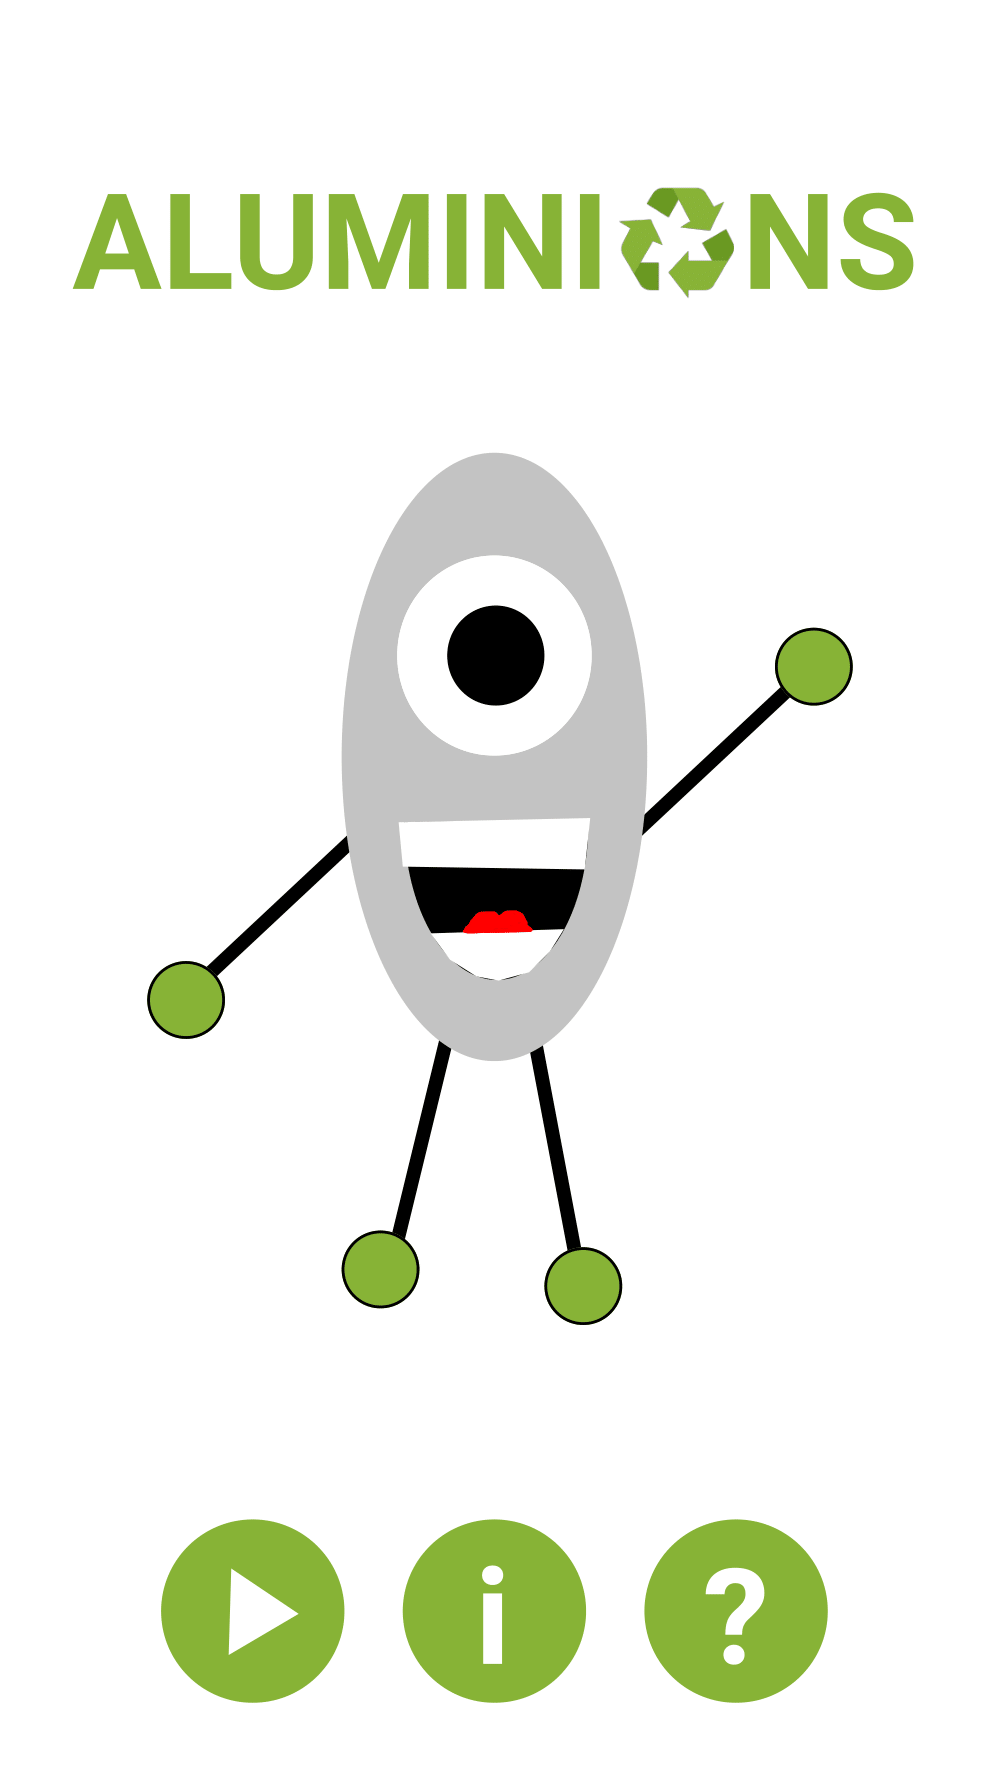
\includegraphics[scale=0.3]{figs/Game Design-03.png}
		\caption{Tela inicial}
	\end{center}
\end{figure}

\begin{figure}[H]
	\begin{center}
		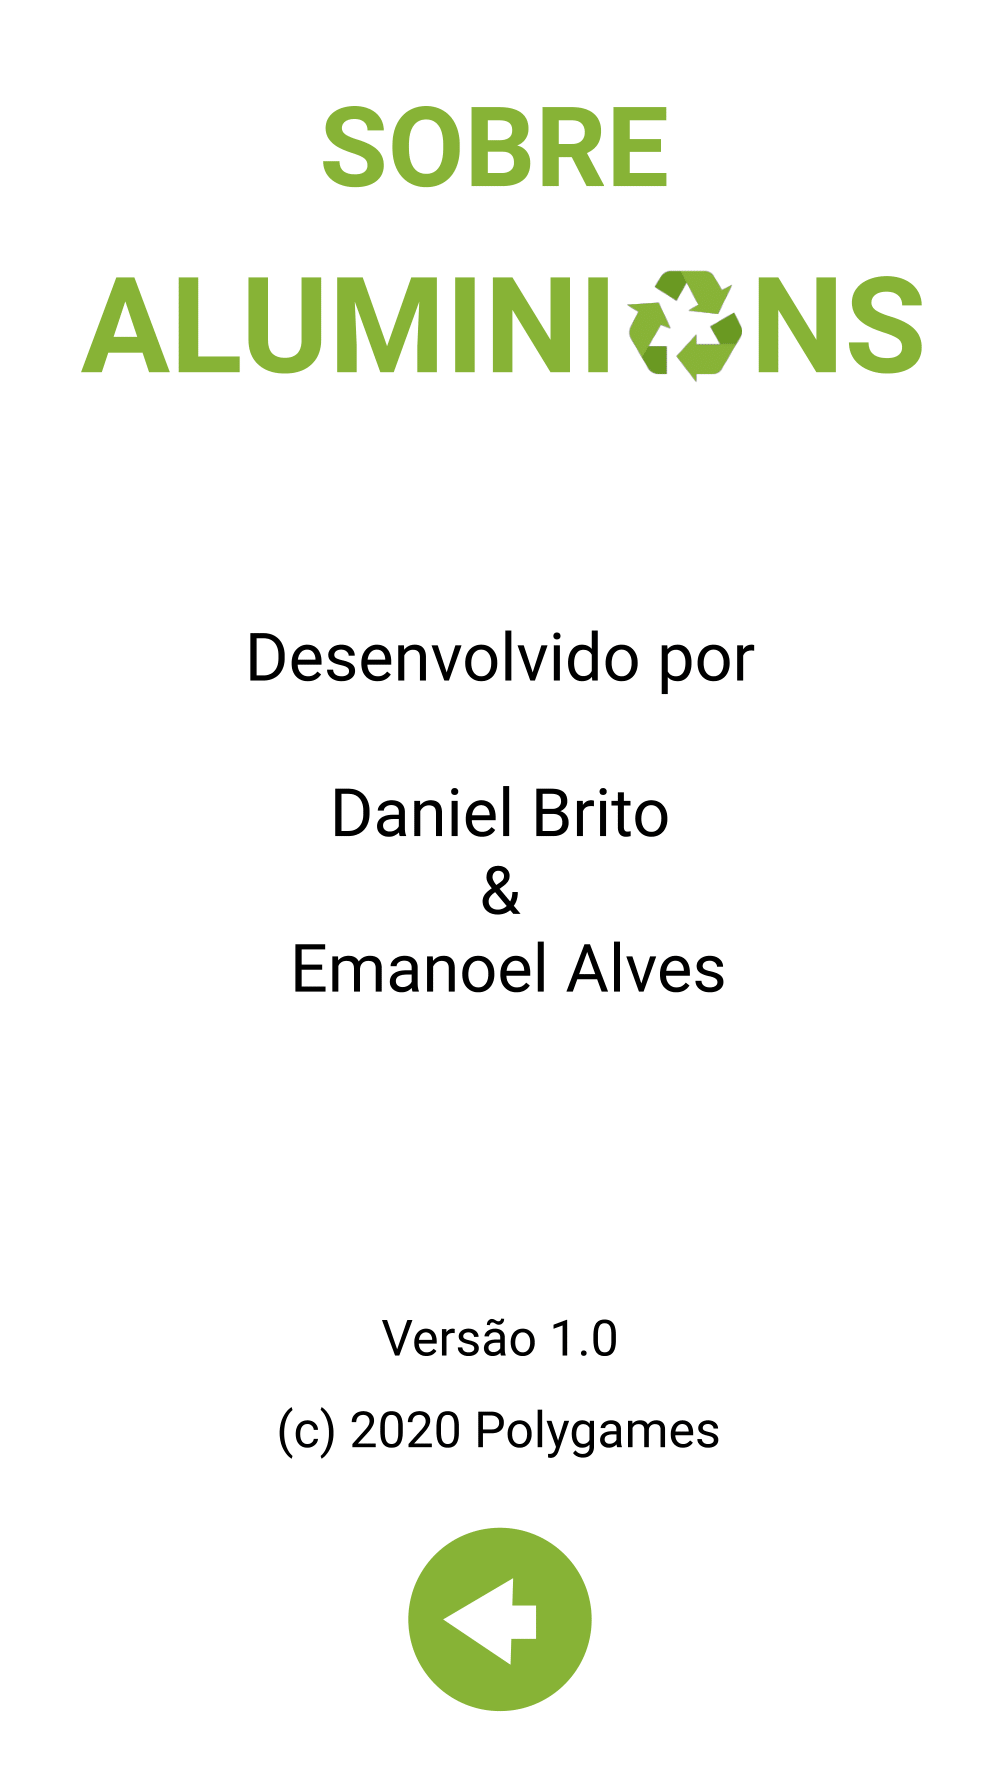
\includegraphics[scale=0.3]{figs/Game Design-18.png}
		\caption{Sobre}
	\end{center}
\end{figure}

\begin{figure}[H]
	\begin{center}
		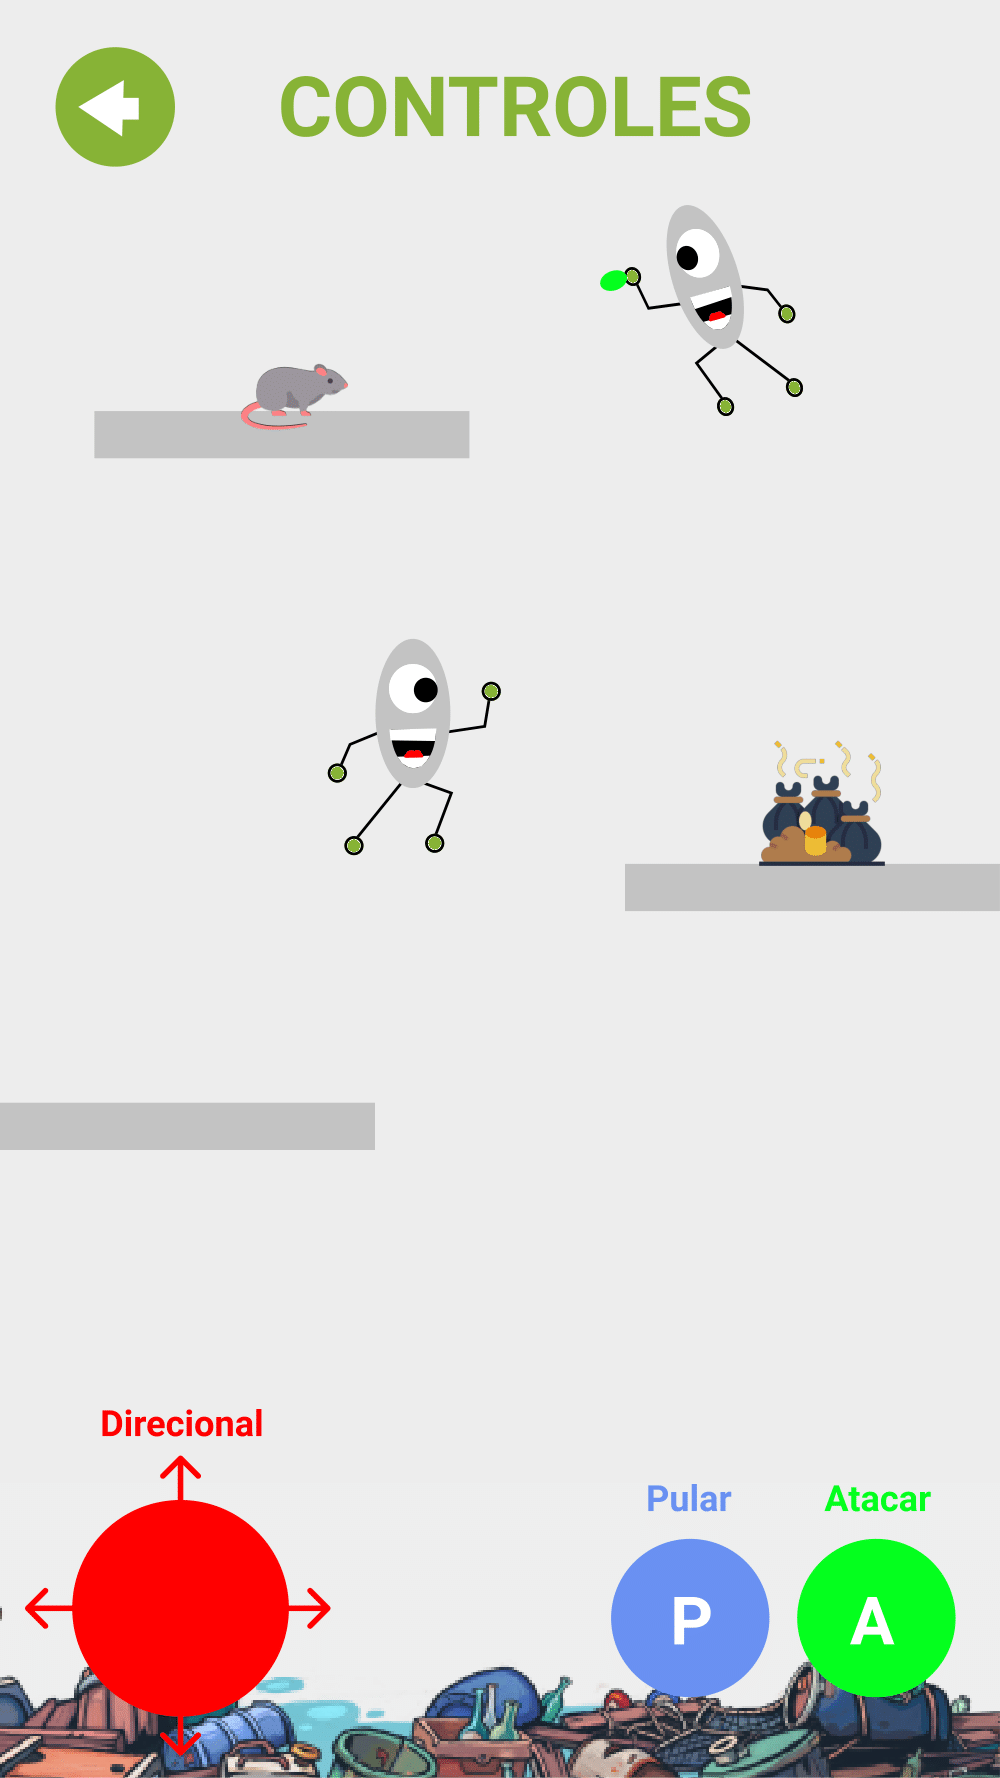
\includegraphics[scale=0.3]{figs/Game Design-19.png}
		\caption{Ajuda}
	\end{center}
\end{figure}

\begin{figure}[H]
	\begin{center}
		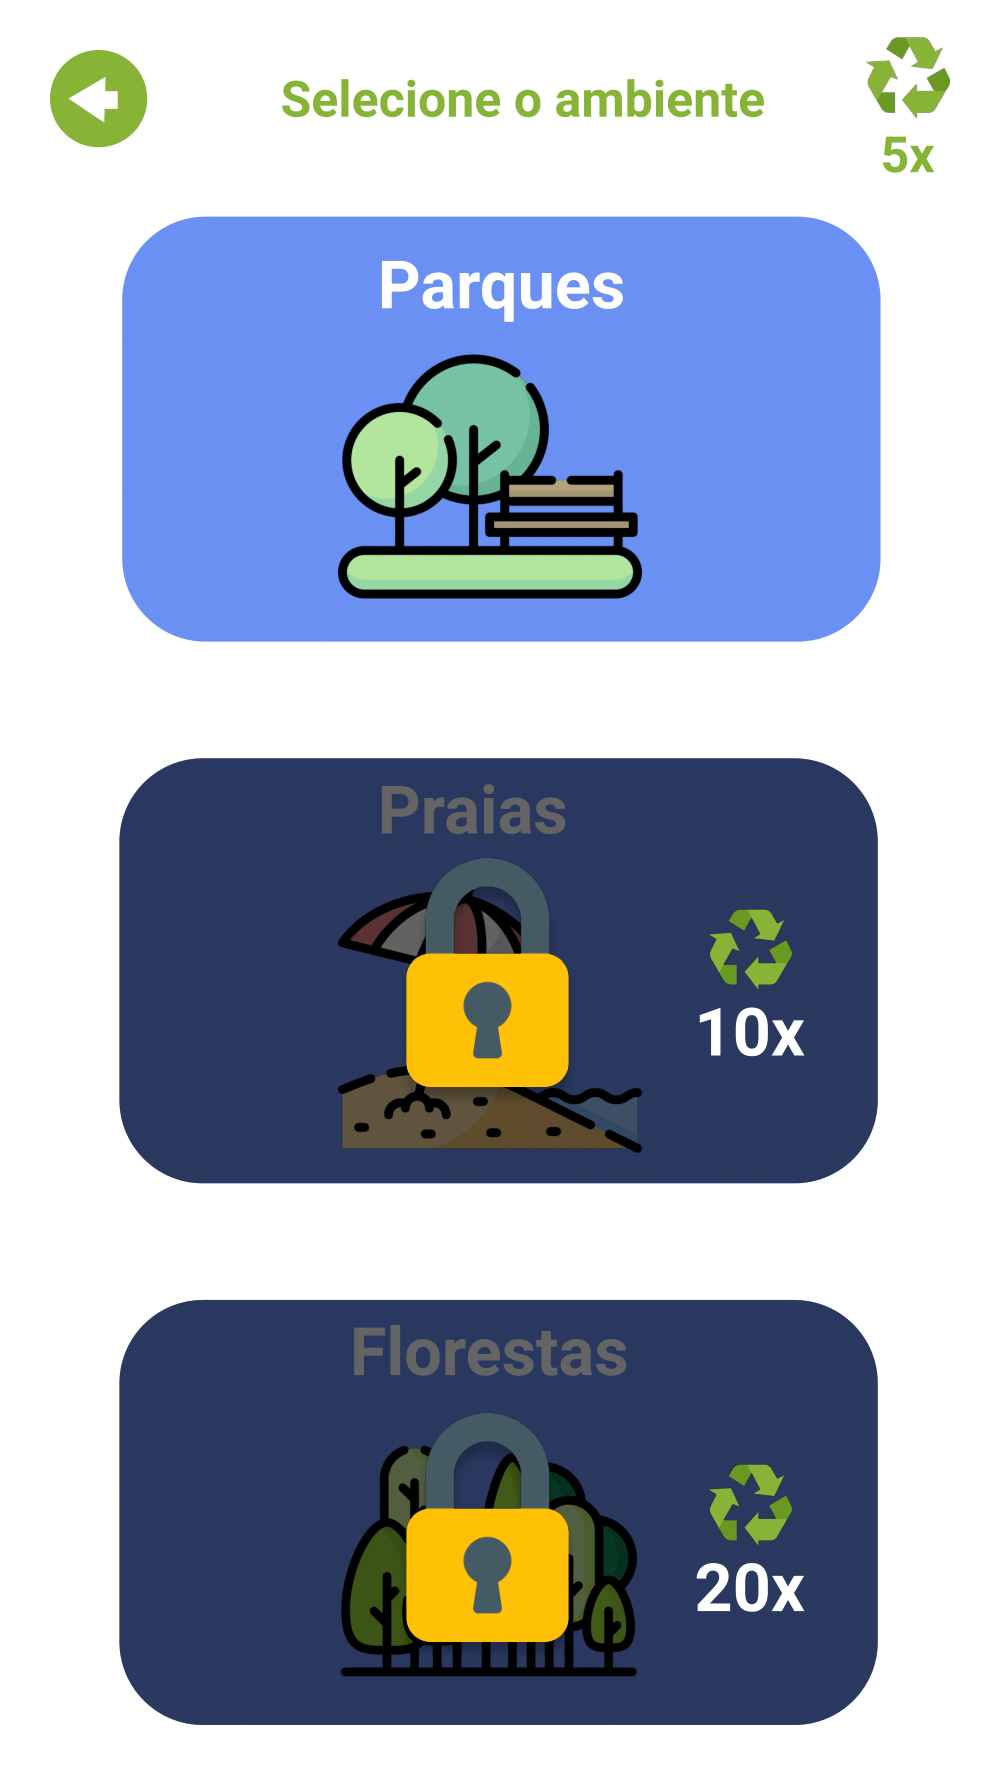
\includegraphics[scale=0.3]{figs/Game Design-04.png}
		\caption{Ambientes}
	\end{center}
\end{figure}

\begin{figure}[H]
	\begin{center}
		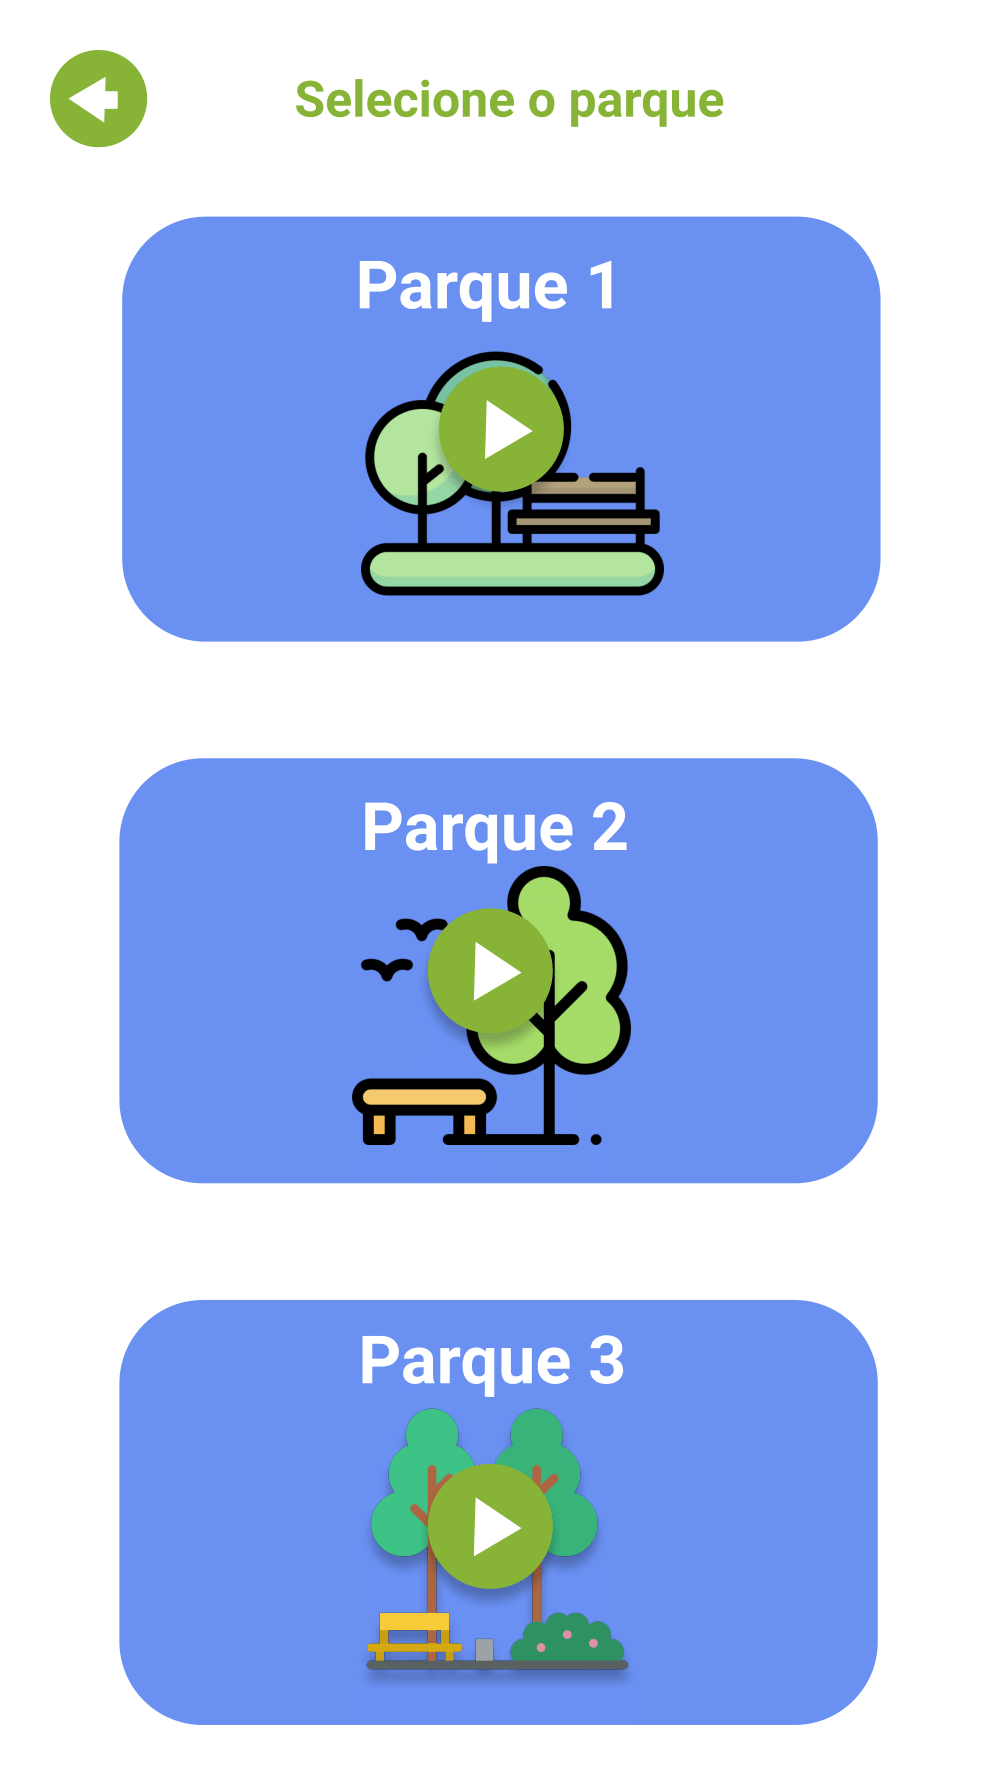
\includegraphics[scale=0.3]{figs/Game Design-05.png}
		\caption{Fases}
	\end{center}
\end{figure}

\begin{figure}[H]
	\begin{center}
		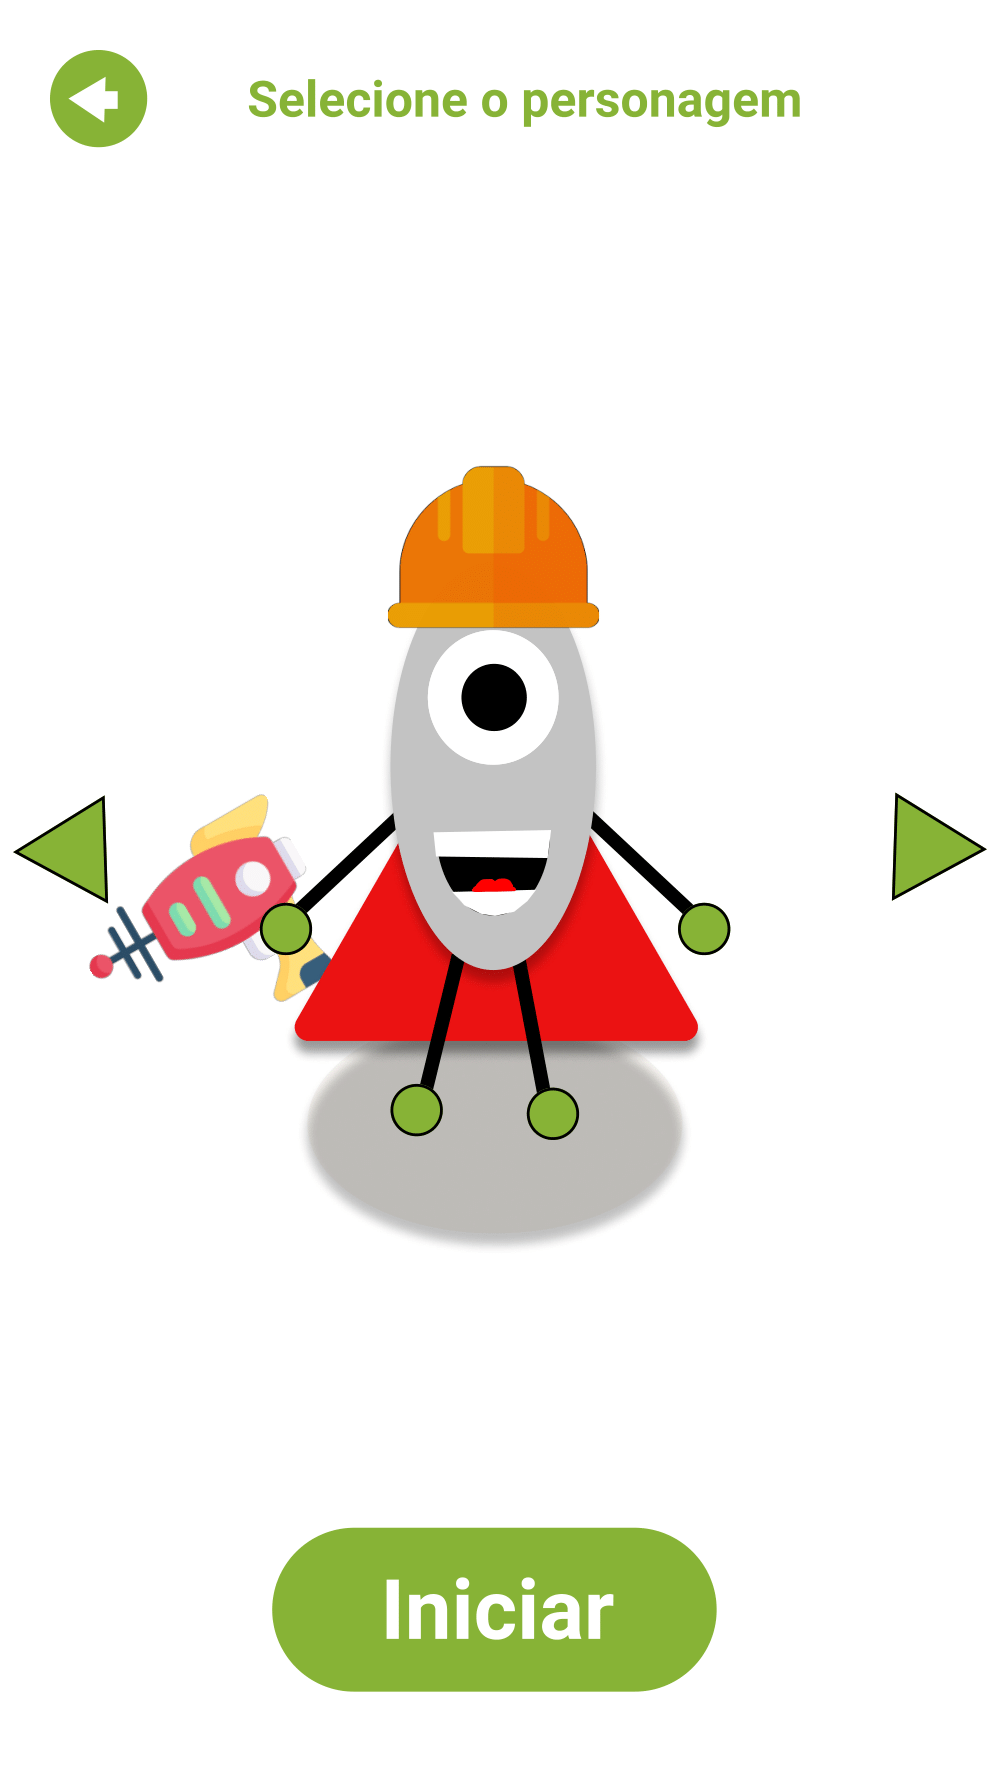
\includegraphics[scale=0.3]{figs/Game Design-06.png}
		\caption{Seleção de avatar}
	\end{center}
\end{figure}

\begin{figure}[H]
	\begin{center}
		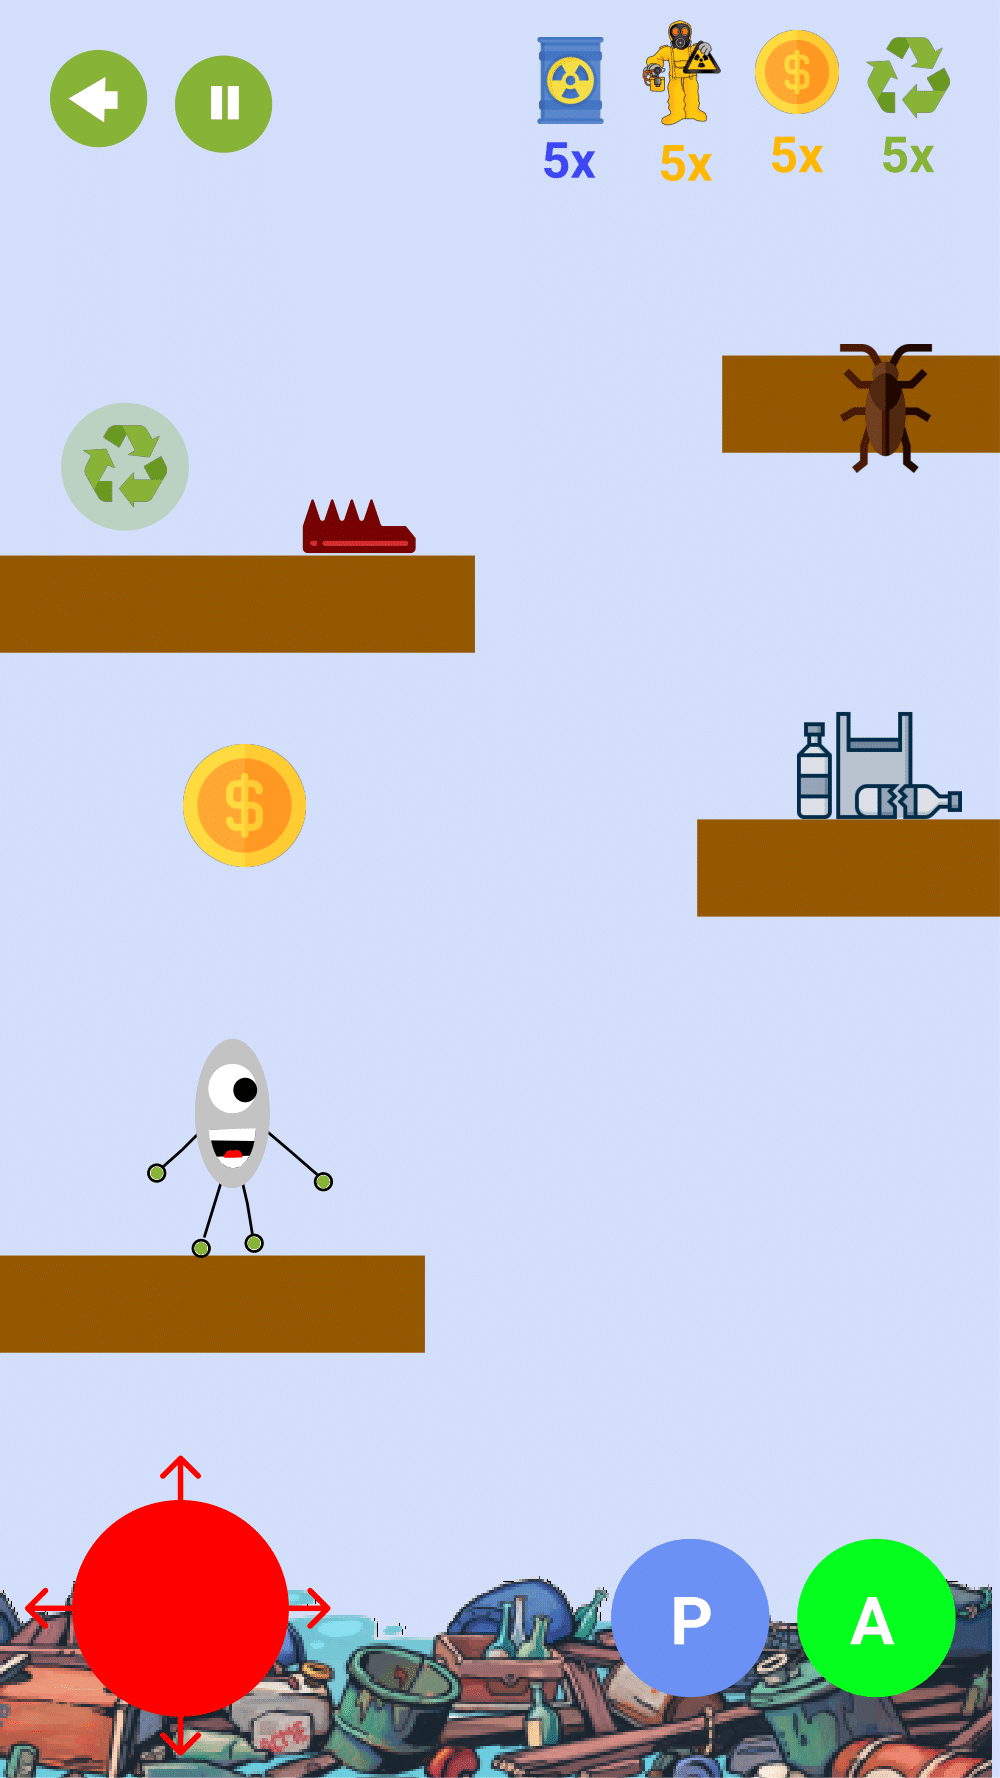
\includegraphics[scale=0.3]{figs/Game Design-07.png}
		\caption{Fase - Praça - Dia}
	\end{center}
\end{figure}

\begin{figure}[H]
	\begin{center}
		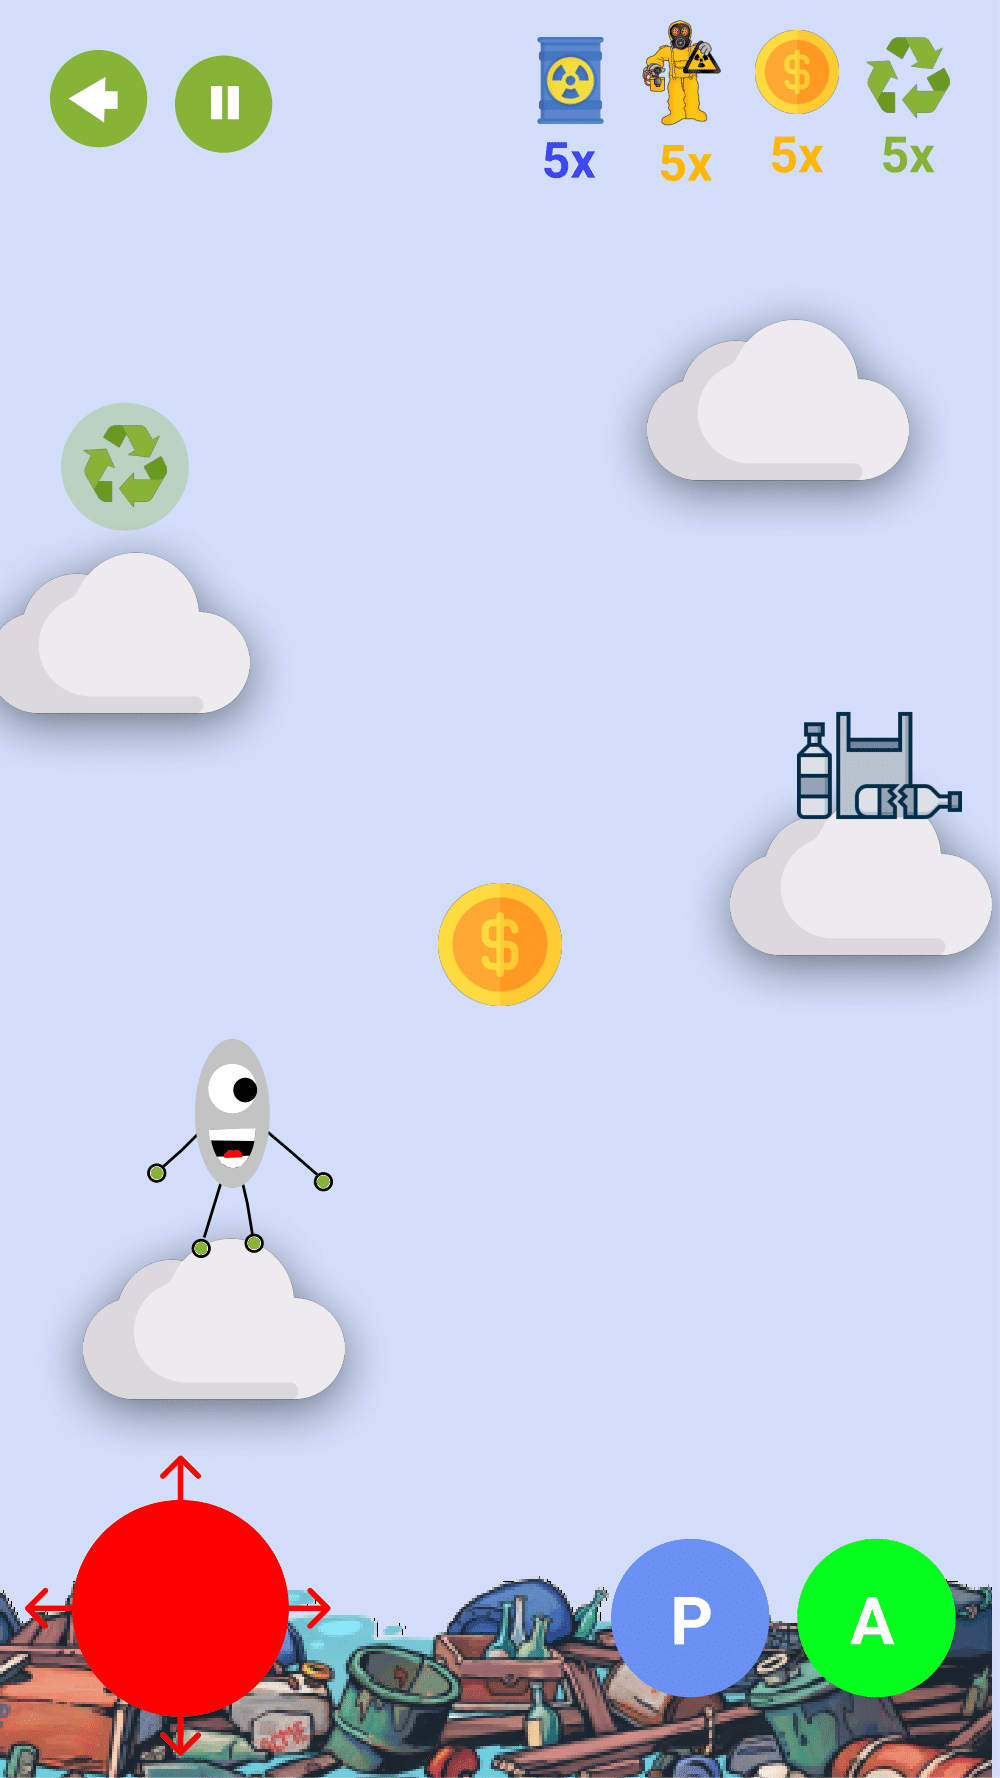
\includegraphics[scale=0.3]{figs/Game Design-08.png}
		\caption{Fase - Praia - Dia}
	\end{center}
\end{figure}

\begin{figure}[H]
	\begin{center}
		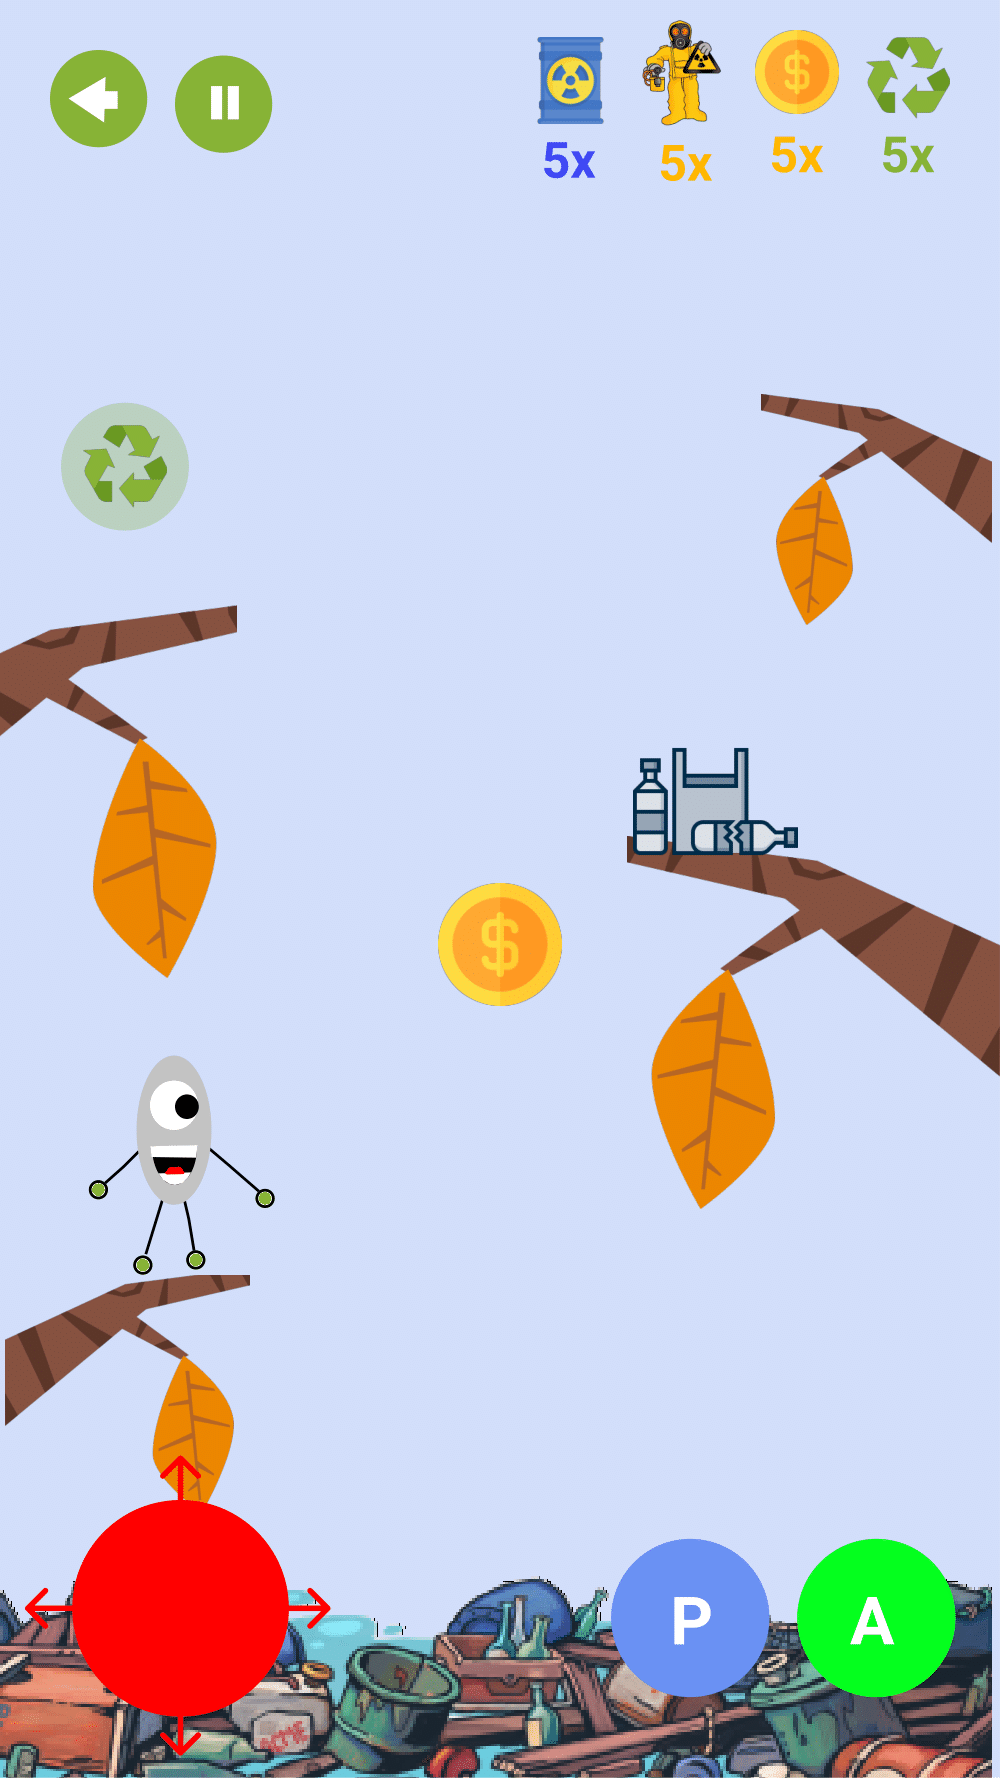
\includegraphics[scale=0.3]{figs/Game Design-09.png}
		\caption{Fase - Floresta - Dia}
	\end{center}
\end{figure}

\begin{figure}[H]
	\begin{center}
		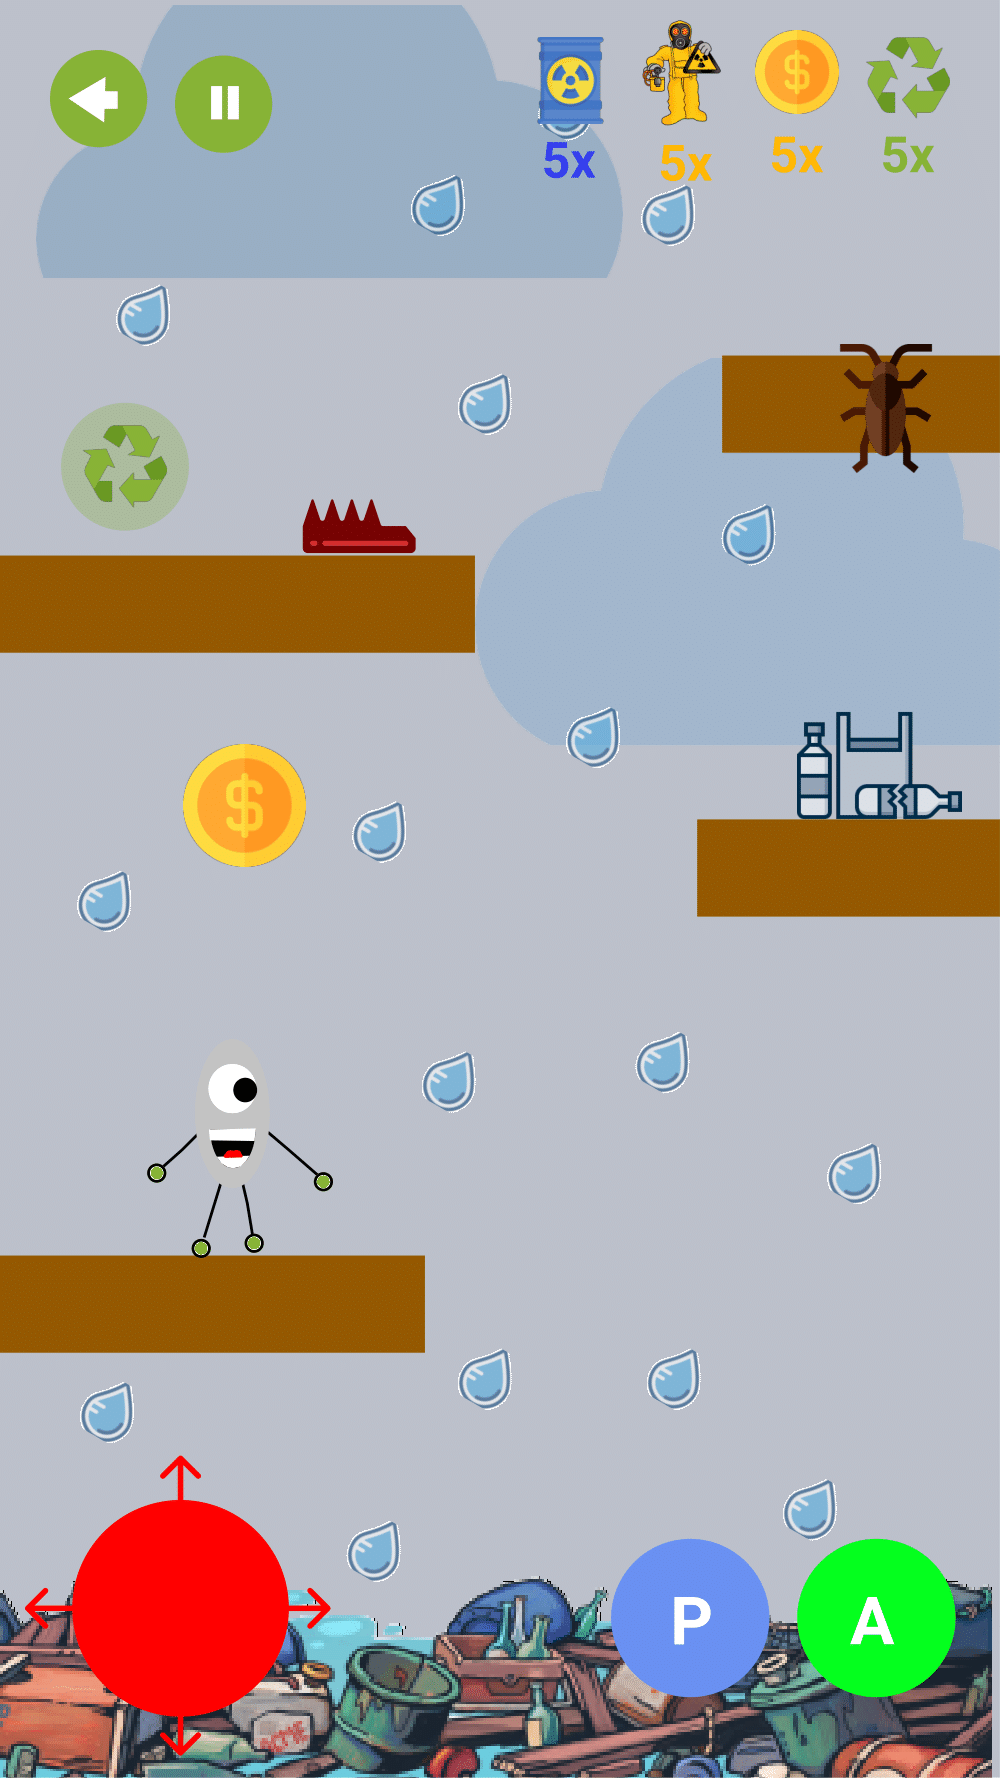
\includegraphics[scale=0.3]{figs/Game Design-10.png}
		\caption{Fase - Praça - Chovendo}
	\end{center}
\end{figure}

\begin{figure}[H]
	\begin{center}
		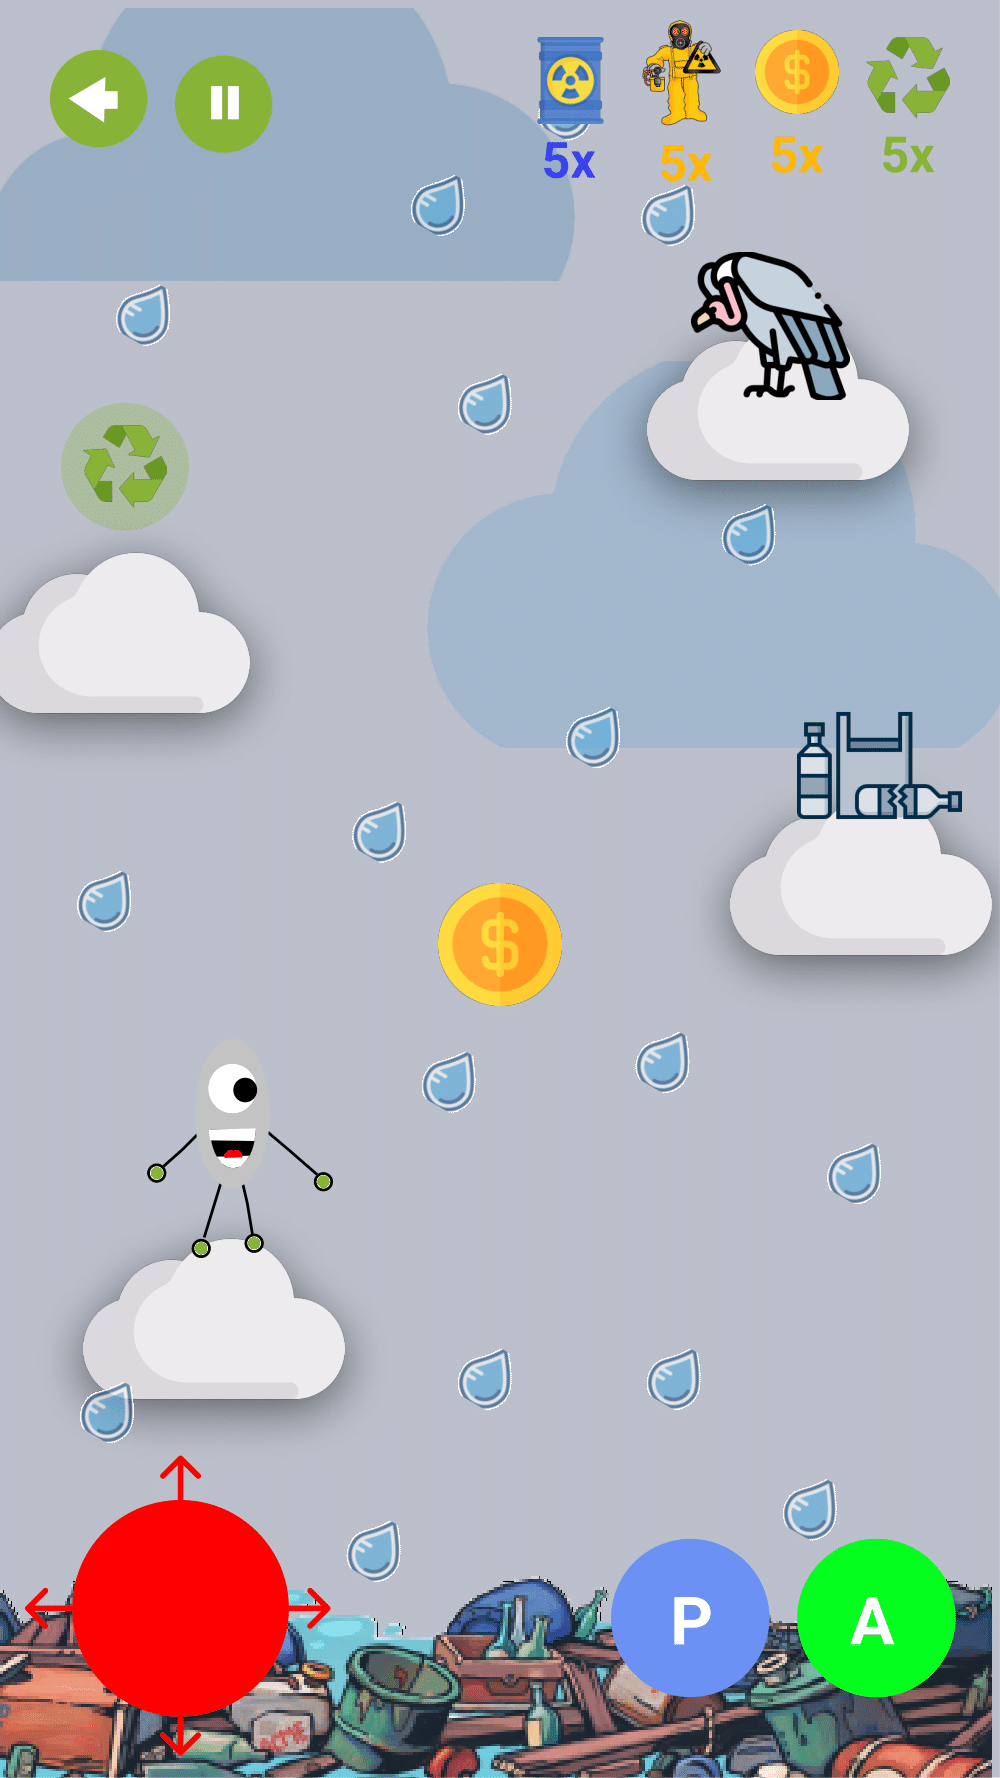
\includegraphics[scale=0.3]{figs/Game Design-11.png}
		\caption{Fase - Praia - Chovendo}
	\end{center}
\end{figure}

\begin{figure}[H]
	\begin{center}
		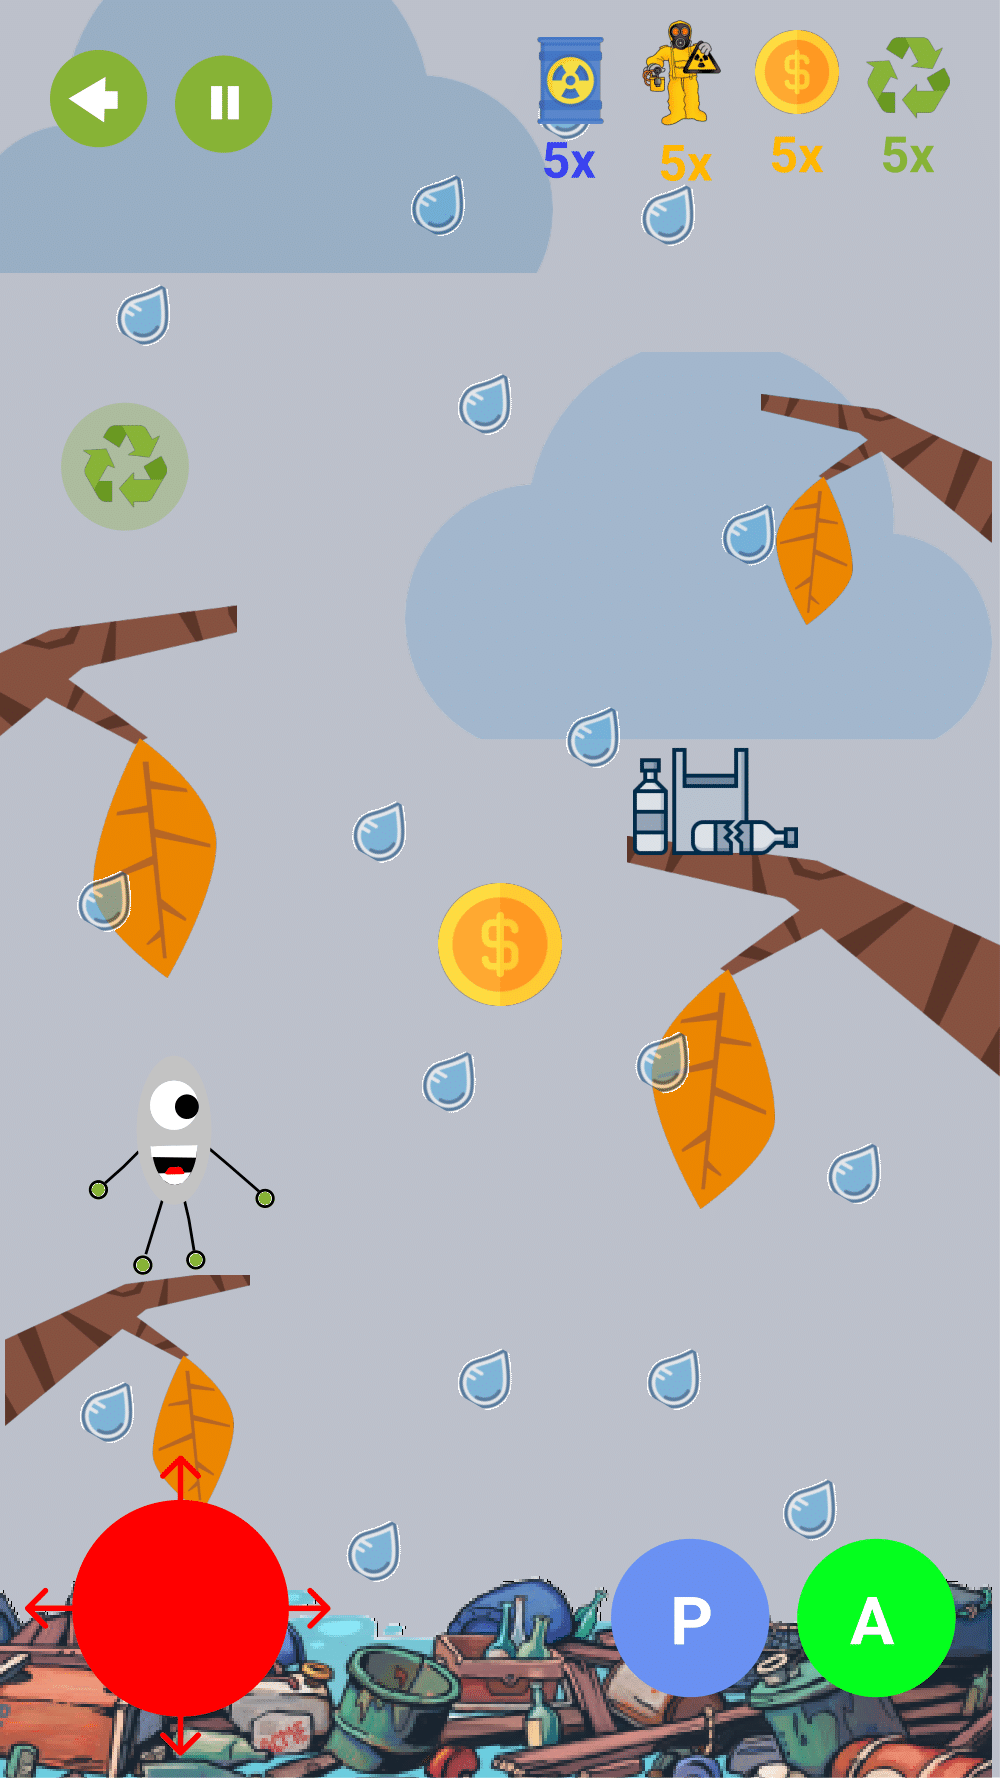
\includegraphics[scale=0.3]{figs/Game Design-12.png}
		\caption{Fase - Floresta - Chovendo}
	\end{center}
\end{figure}

\begin{figure}[H]
	\begin{center}
		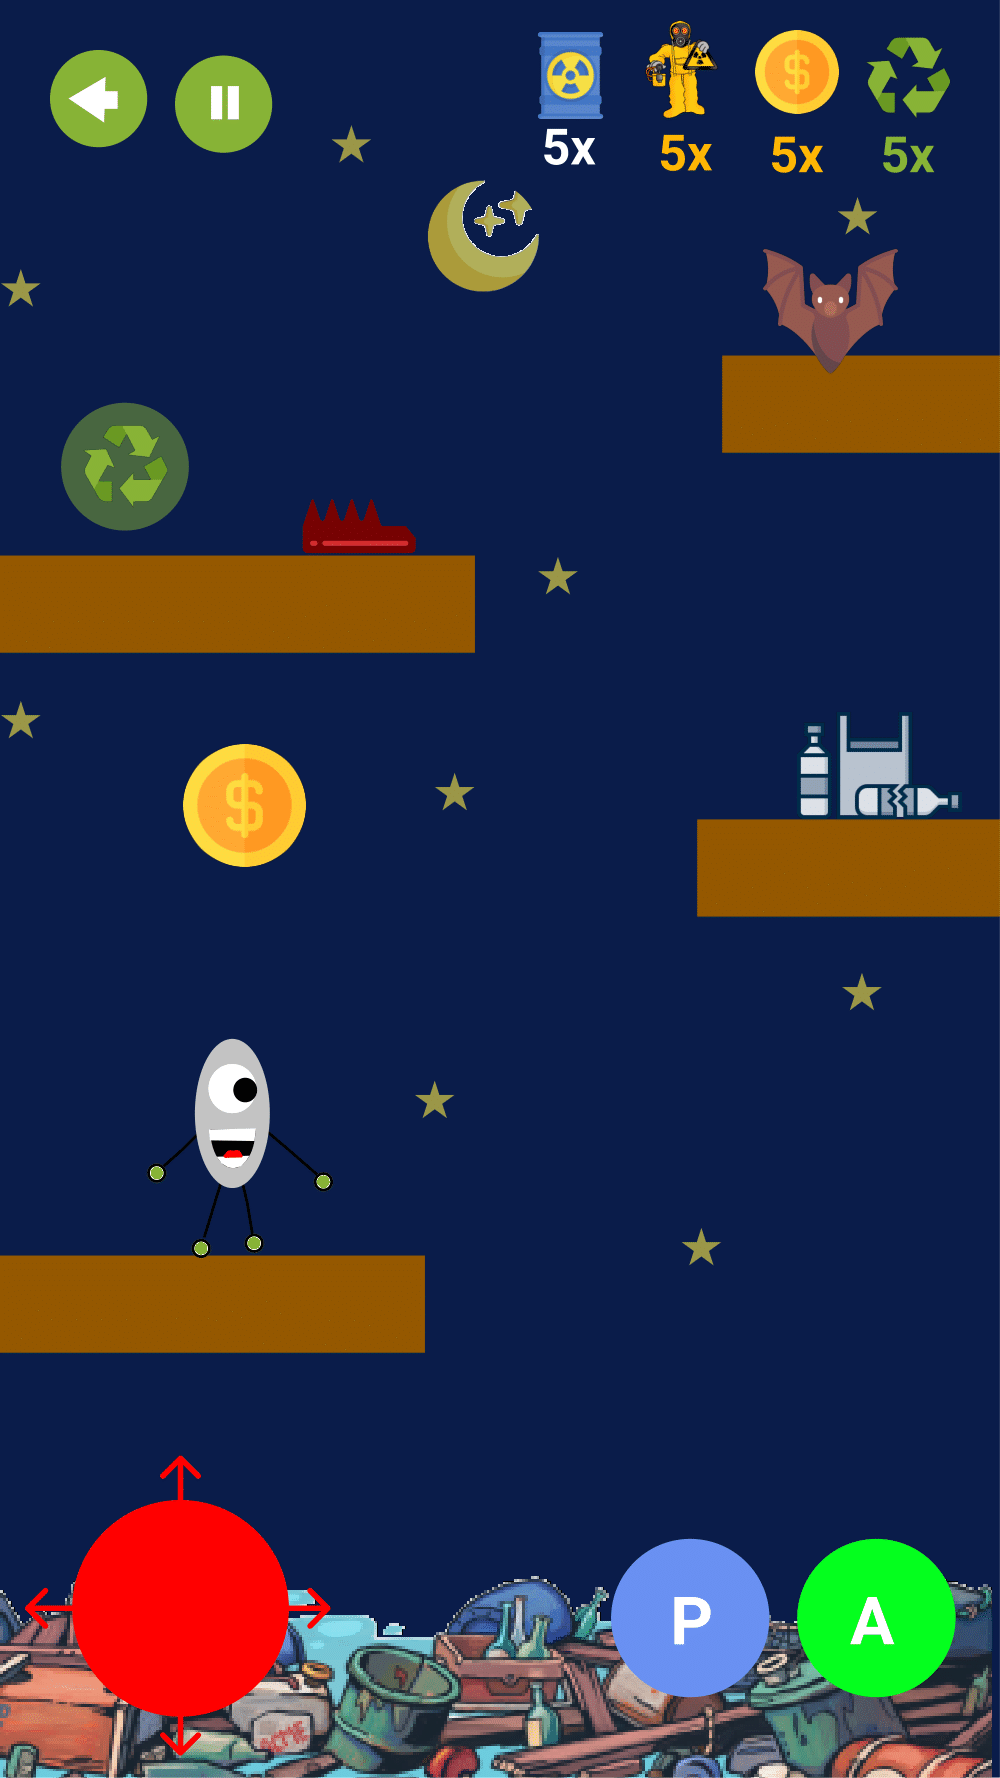
\includegraphics[scale=0.3]{figs/Game Design-13.png}
		\caption{Fase - Praça - Noite}
	\end{center}
\end{figure}

\begin{figure}[H]
	\begin{center}
		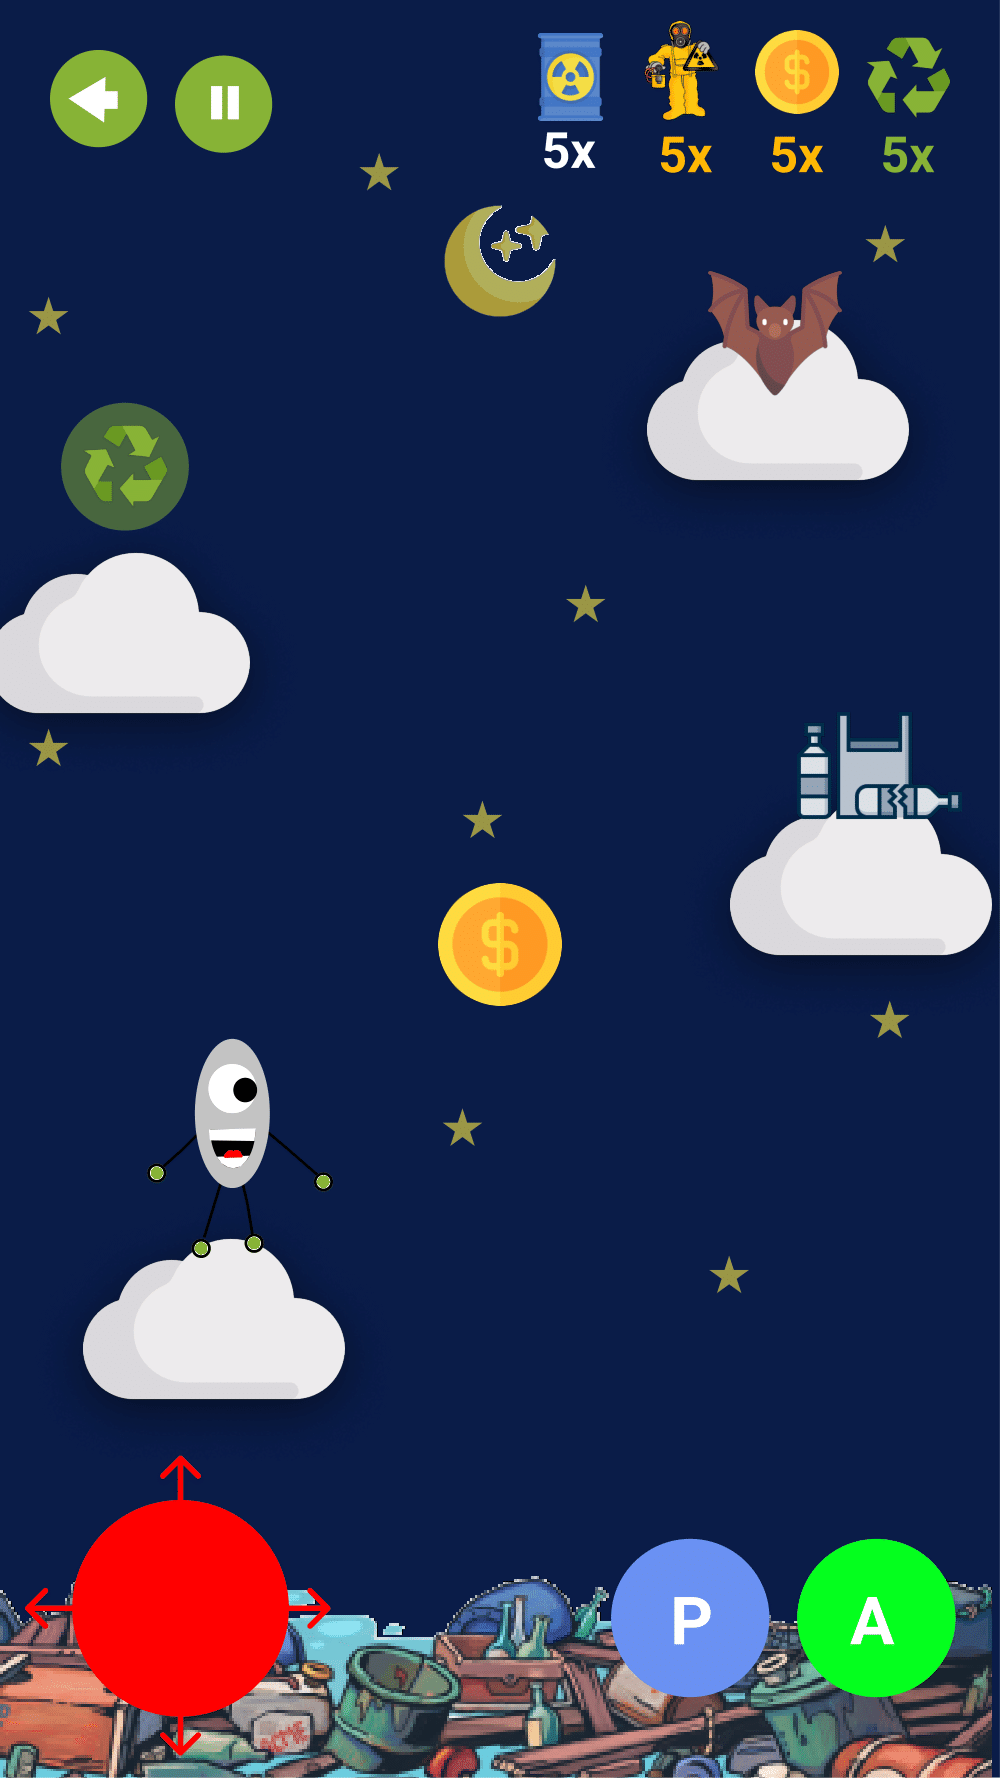
\includegraphics[scale=0.3]{figs/Game Design-14.png}
		\caption{Fase - Praia - Noite}
	\end{center}
\end{figure}

\begin{figure}[H]
	\begin{center}
		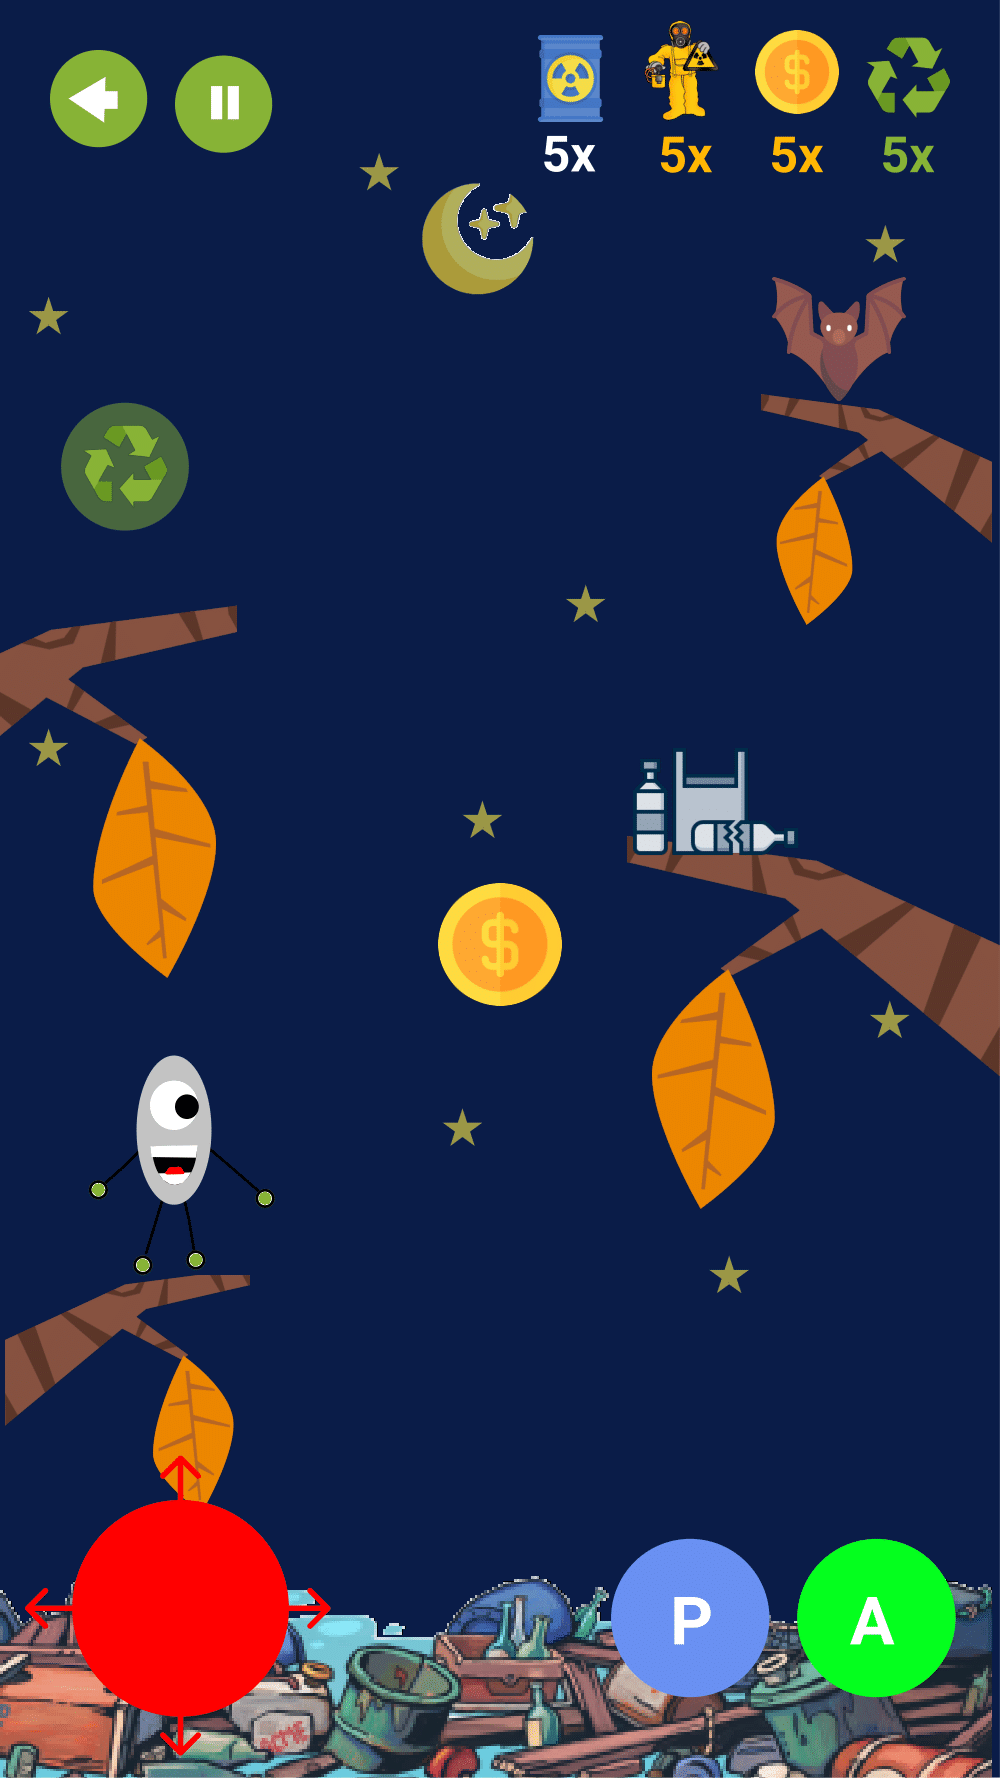
\includegraphics[scale=0.3]{figs/Game Design-15.png}
		\caption{Fase - Floresta - Noite}
	\end{center}
\end{figure}

\begin{figure}[H]
	\begin{center}
		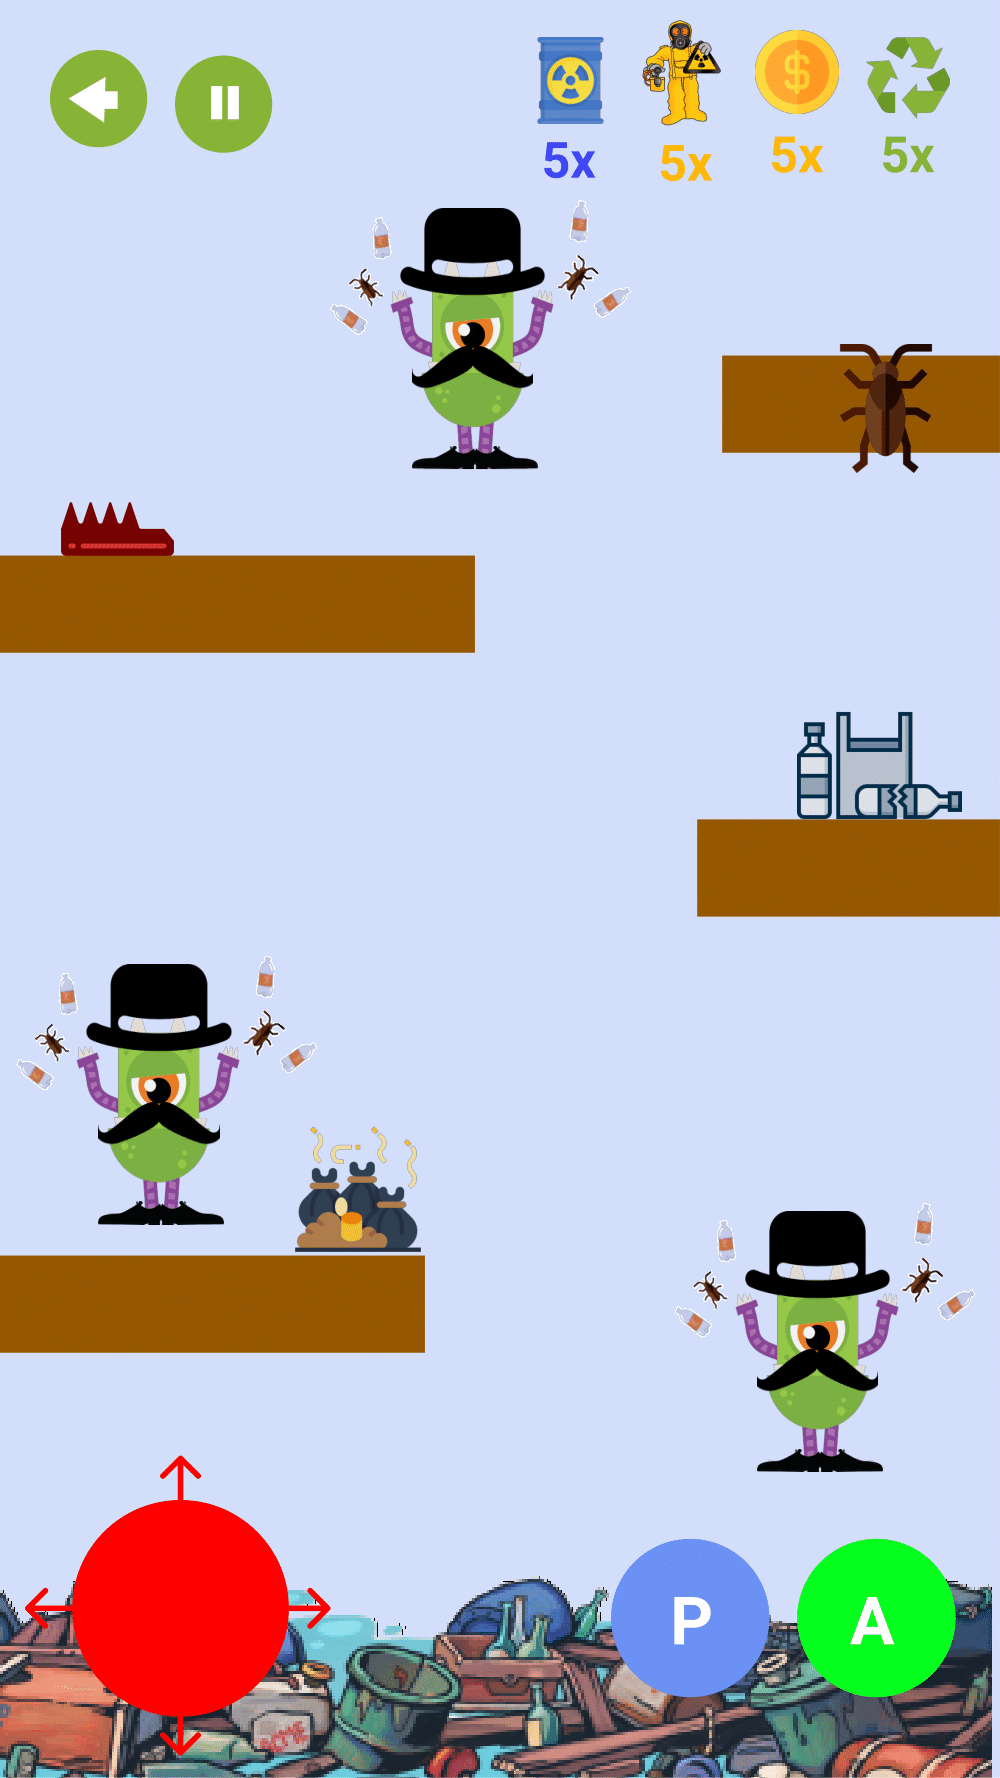
\includegraphics[scale=0.3]{figs/Game Design-16.png}
		\caption{Luiz Espalha Lixo - Praça}
	\end{center}
\end{figure}

\begin{figure}[H]
	\begin{center}
		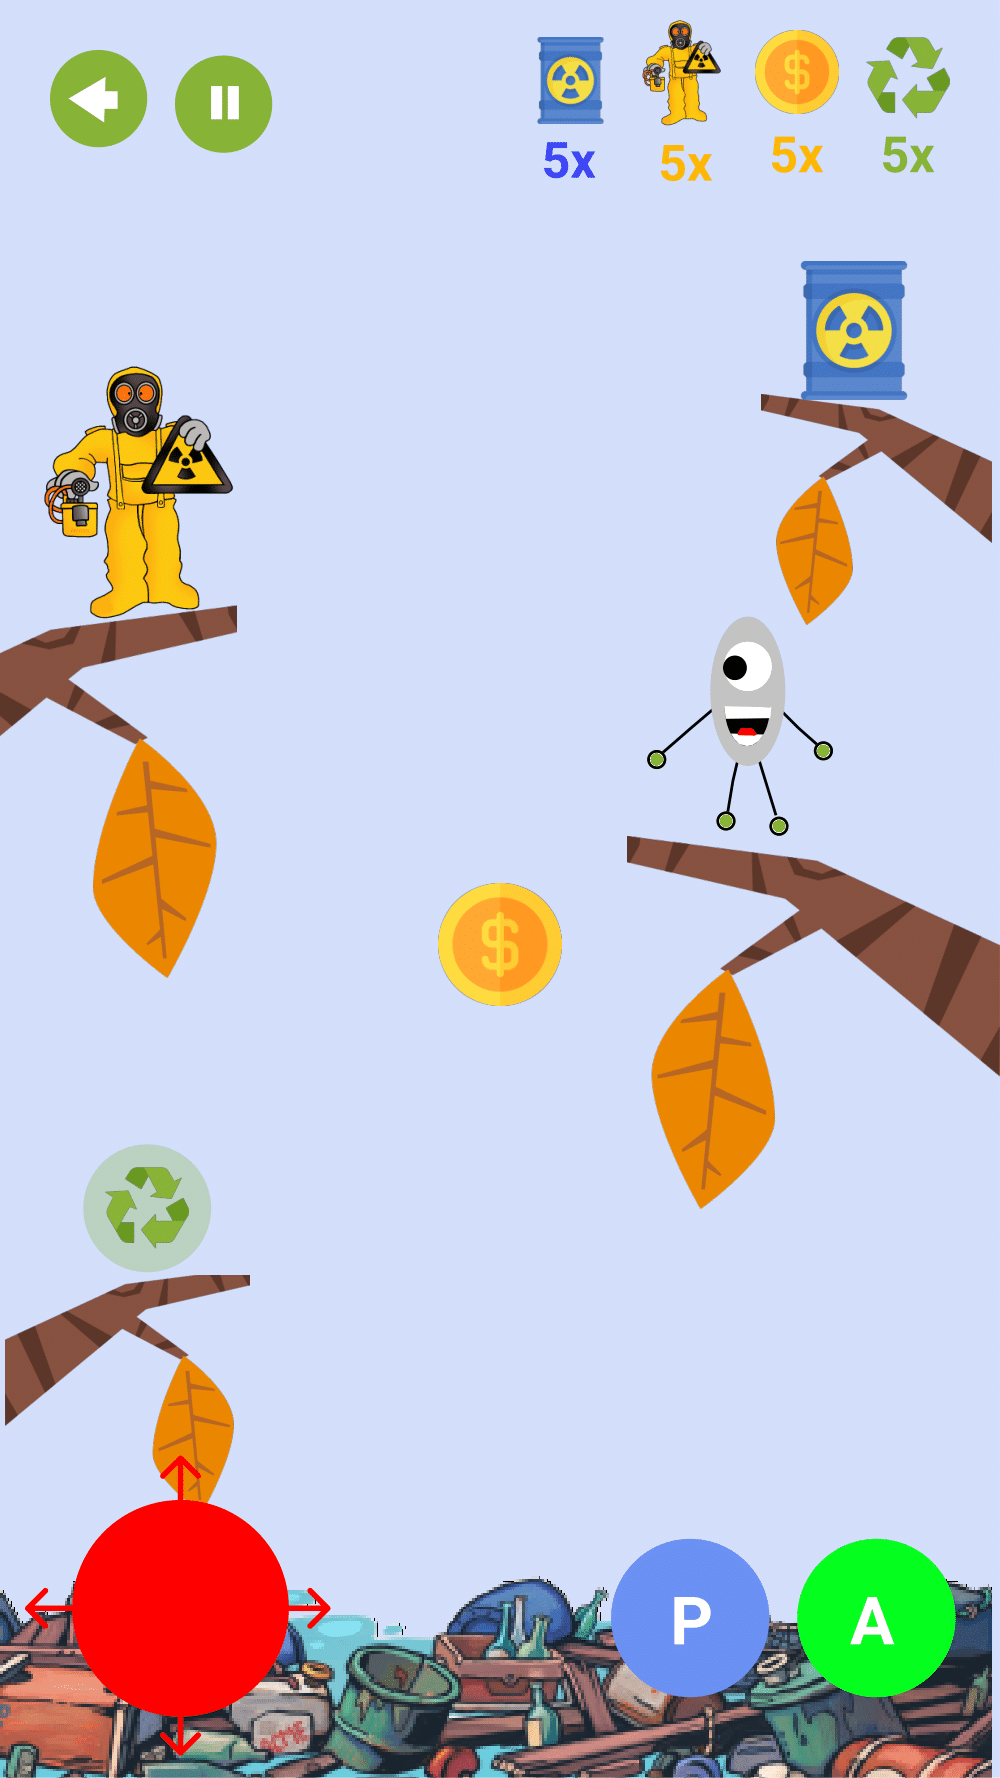
\includegraphics[scale=0.3]{figs/Game Design-17.png}
		\caption{Luiz Espalha Lixo - Floresta}
	\end{center}
\end{figure}

\begin{figure}[H]
	\begin{center}
		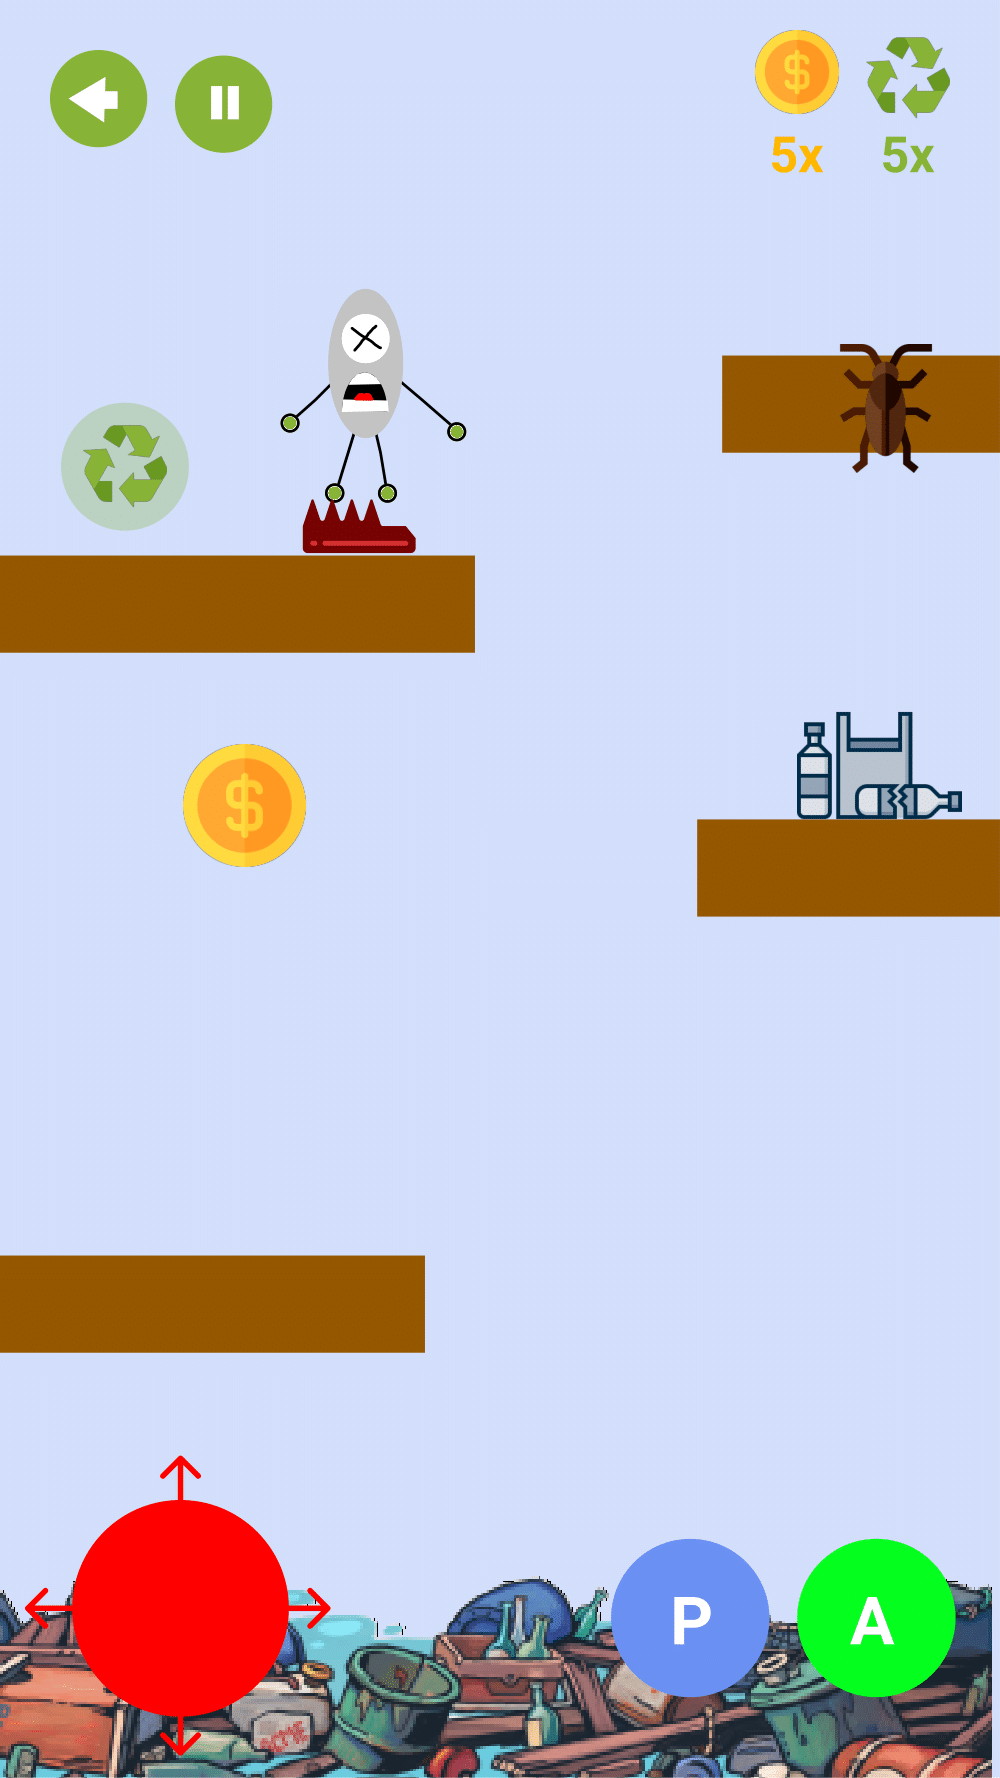
\includegraphics[scale=0.3]{figs/Game Design-01.png}
		\caption{Game Over - Armadilha}
	\end{center}
\end{figure}

\begin{figure}[H]
	\begin{center}
		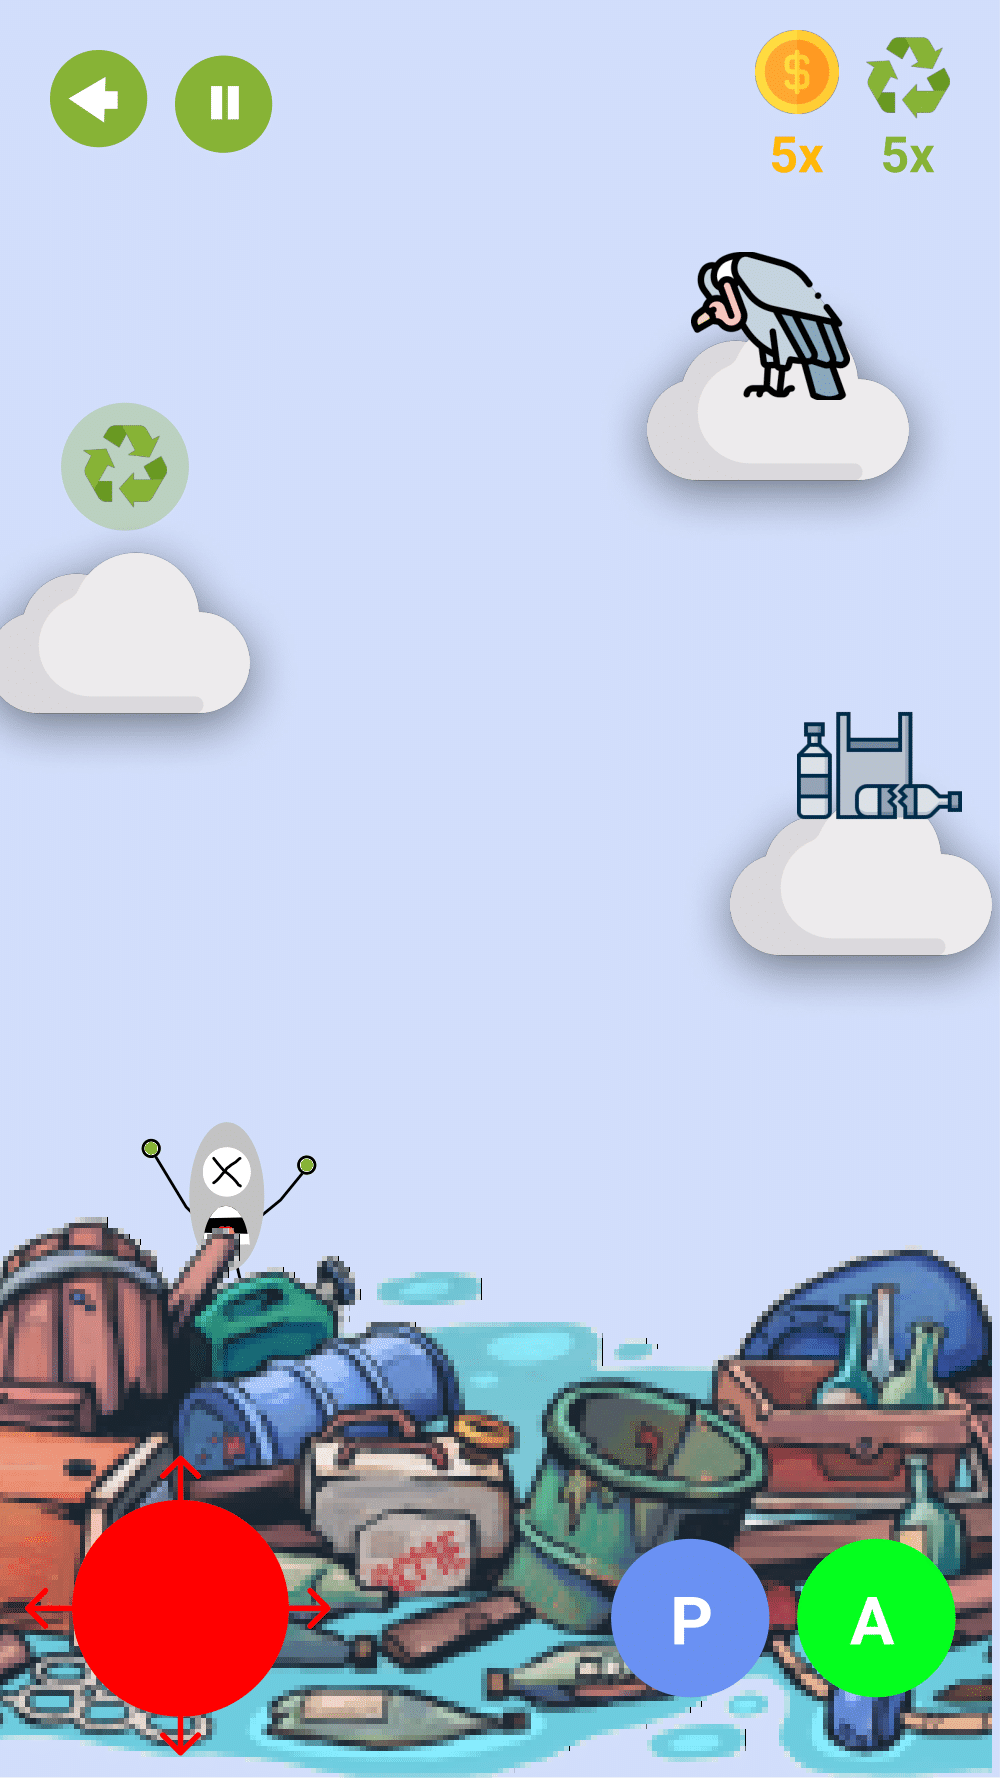
\includegraphics[scale=0.3]{figs/Game Design-02.png}
		\caption{Game Over - Afogado}
	\end{center}
\end{figure}

\begin{figure}[H]
	\begin{center}
		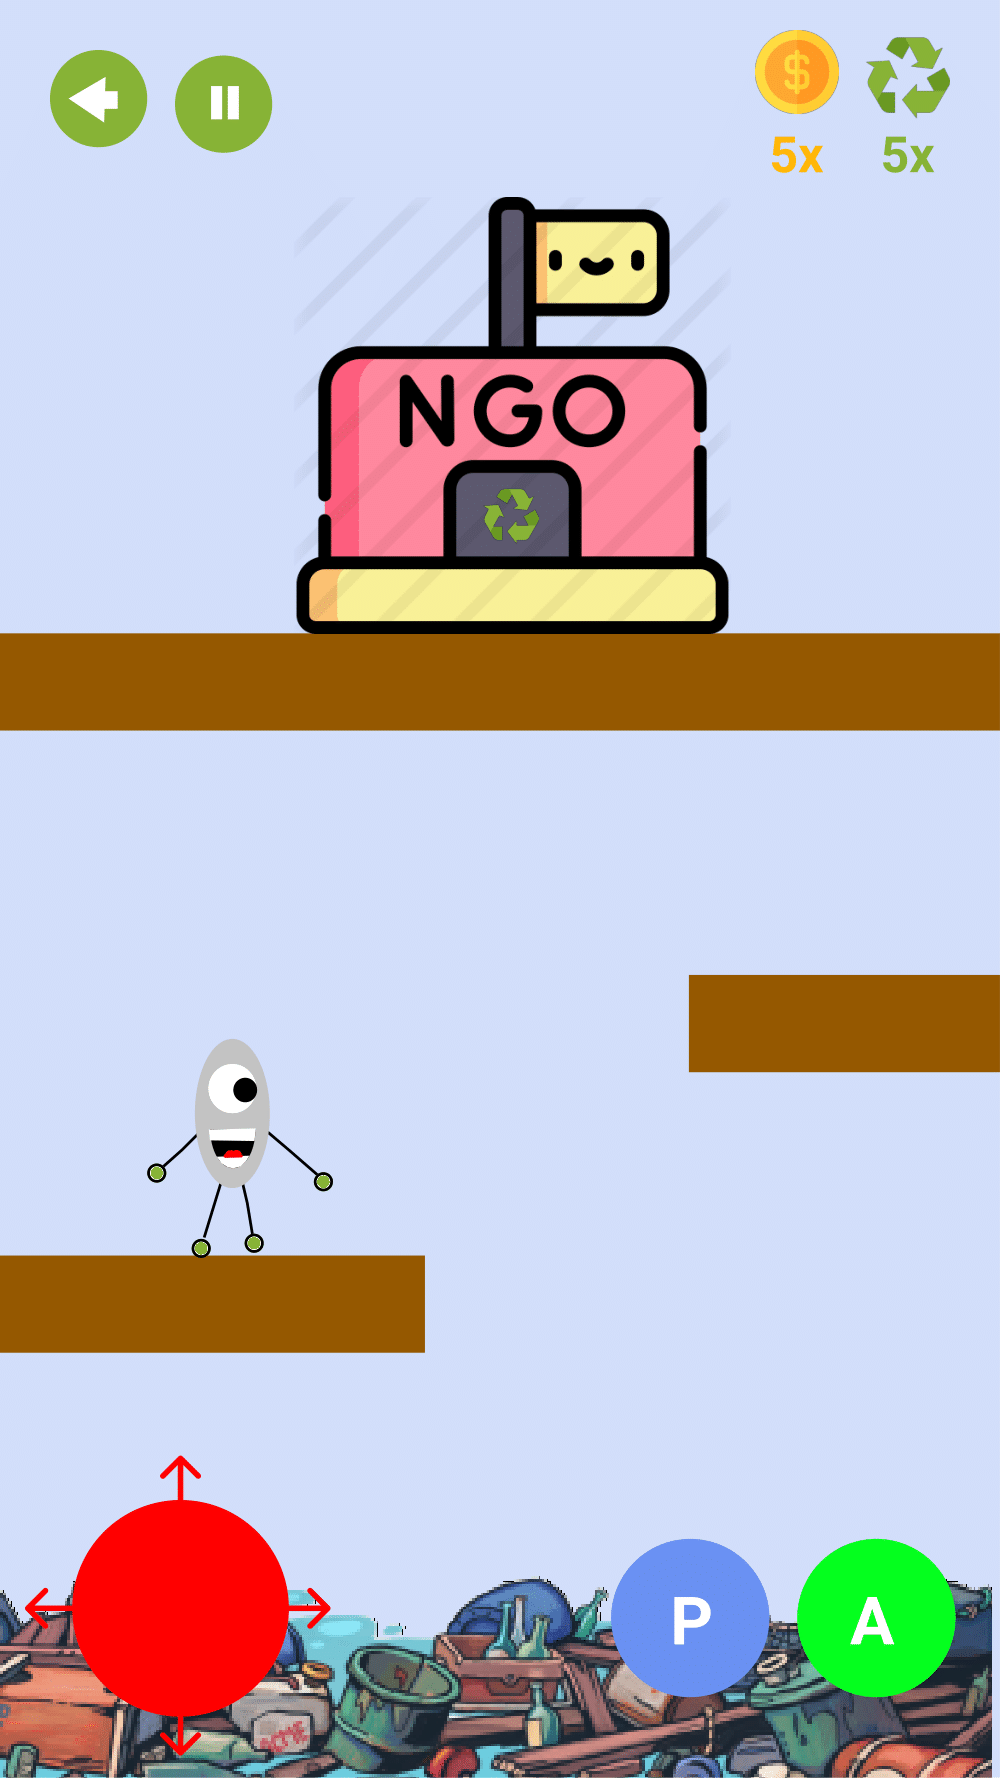
\includegraphics[scale=0.3]{figs/Game Design-20.png}
		\caption{ONG Reciclope}
	\end{center}
\end{figure}

\begin{figure}[H]
	\begin{center}
		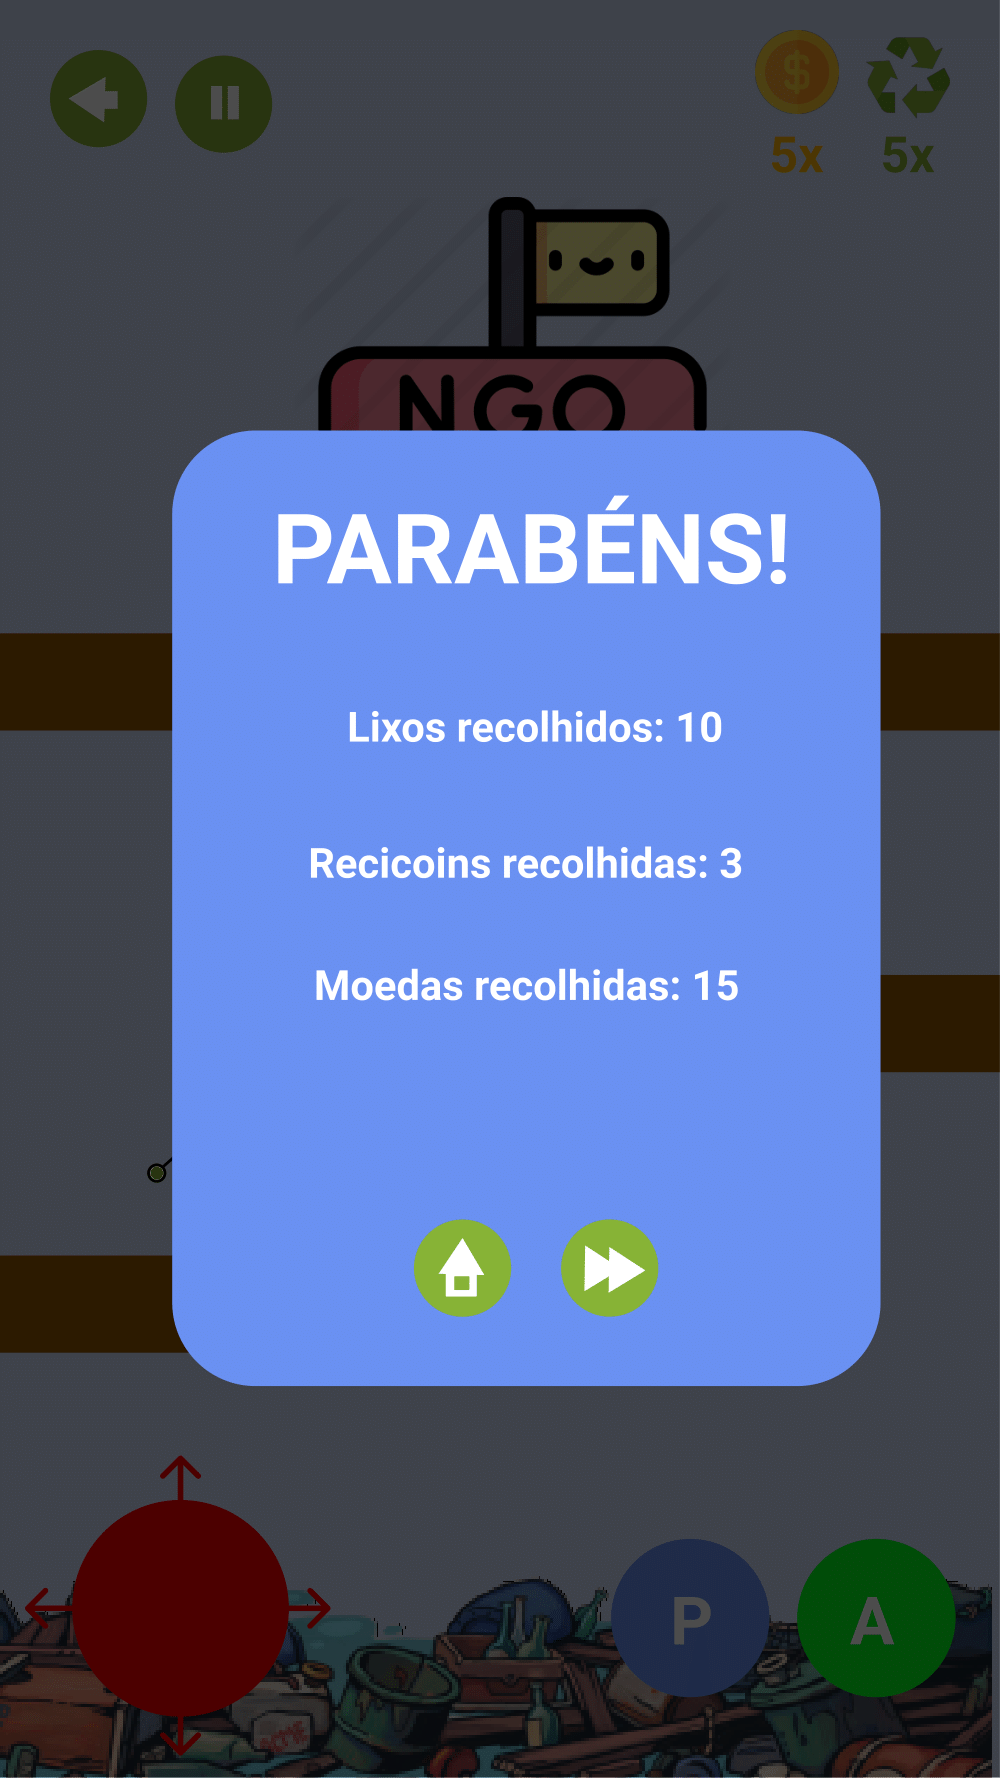
\includegraphics[scale=0.3]{figs/Game Design-21.png}
		\caption{Game Over - Parabenização}
	\end{center}
\end{figure}

\noindent\textbf{Quais as funcionalidades dos itens da interface (botões, caixas de texto)?}

\textbf{Botão de informação:} Mostra as informações do jogo, como desenvolvedores e versão.

\textbf{Botão de play:} Inicia a partida.

\textbf{Botão de ajuda:} Mostra os controles.

\textbf{Botão de voltar:} Retorna para a tela anterior.

\textbf{Imagens de categorias:} Exibe as respectivas fases.

\textbf{Botão direcional vermelho:} Movimenta o Aluminion.

\textbf{Botão azul:} Pula.

\textbf{Botão verde limão:} Atira.

\textbf{Botão de pause:} Pausa a partida.

\textbf{Botão de home:} Retorna para o menu de fases.

\textbf{Botão de avançar:} Inicia a próxima partida.

\section{Personagens}

\subsection{Descrição de todos os personagens do jogo}

\noindent\textbf{Nome:} Aluminion

\noindent\textbf{Aspectos físicos e personalidade:} Arredondado, ciclópico, de alumínio e engajado em causas ambientais.

\noindent\textbf{Atributos:} Capacete, pistola e outros, a depender da skin.

\noindent\textbf{História:} Os Aluminions são pequenas criaturas formadas por lacres de alumínio que foram criados para ajudar na limpeza de áreas ambientais. Com essa motivação, estão dispostos a enfrentar uma diversidade de obstáculos para contribuírem com as causas ambientais.

\noindent\textbf{Relação com outros personagens:} Inimizade.

\subsection{Lista de todos os personagens controlados pelo jogador}

Apenas o Aluminion.

\subsection{Lista de todos os personagens não controlados pelo jogador}

\noindent\textbf{Inimigos:} Ratazanas, morcegos, “Luiz Espalha Lixo”, baratas, urubus.

\noindent\textbf{Aliados e amigos:} Não.

\noindent\textbf{Neutros:} Não.

\noindent\textbf{Comportamentos de inteligência artificial:} Não.

\section{História}

\subsection{Resumo da história em até 2 parágrafos}

Em um mundo onde cada vez mais pessoas poluem parques, praias, florestas e outras áreas ambientais, foi idealizada a criação de uma criatura para ajudar na preservação do meio-ambiente. Os Aluminions, como são chamados, foram criados para recolher os resíduos espalhados por diversos ambientes, e levar para a ONG de reciclagem Reciclope.

\subsection{História completa}

\noindent\textbf{Justificativa da história. O que ocorreu para o início dos fatos da história?}

Os integrantes da ONG Reciclope decidiram que a criação de ajudantes para recolher os resíduos descartados pelos pessoas e o vilão “Luiz espalha lixo”, seria uma boa forma de otimizar o processo de preservação do meio-ambiente.

\noindent\textbf{Liste todos os acontecimentos da história.}

Poluição do meio ambiente.

Criação de criatura para prevenção do meio ambiente.

Reciclagem de lixo pelas ONGs.

\noindent\textbf{Em que período a história ocorrerá?}

No presente.

\noindent\textbf{Quais as consequências dos acontecimentos da história?}

No final, o mundo será um lugar muito mais saudável de se viver.

\noindent\textbf{Quais os pequenos acontecimentos que ocorrem na história?}

Antes de começar o jogo, o inimigo “Luiz Espalha Lixo’, sai espalhando lixo pelas plataformas. Além disso, devido à chuva e ao lixo, a maré está subindo cada vez mais rápido.

\subsection{Formas de narração da história (diálogos, monólogos)?}

Não tem.

\section{Mundo}

\subsection{Descrição detalhada dos elementos que compõem o mundo
do jogo}

\noindent\textbf{Mapa}

O mapa é dividido em categorias (parques, praias e florestas), então, em cada categoria estão presentes as respectivas fases.

\noindent\textbf{O mapa será grande, médio ou pequeno e por quê?}

Médio, pois o desenrolar do jogo não é muito extenso.

\noindent\textbf{Pontos importantes do mapa (cidades, castelos, regiões, rios, montanhas, etc).}

Parques, florestas, praias e ONGs.

\noindent\textbf{Como o jogador se deslocará no mapa? (caminhando, veículos, animais, teletransporte)}

Pulando e andando.

\noindent\textbf{Quais as condições climáticas do mundo?}

Ensolarado, Chuvoso.

\noindent\textbf{Existirá mudanças de dia e noite? Em tempo real? Qual a
velocidade das mudanças?}

Sim. Não. Nenhuma especificamente, algumas serão de dia e outras de noite, alternadamente.

\noindent\textbf{Como a física é no mundo? (gravidade, densidade de líquidos, etc)}

Normal.

\noindent\textbf{Quais as raças e divisões sociais?}

Aluminions, Luiz Espalha Lixo, humanos (ONGs).

\noindent\textbf{Quais os costumes do povo? Eles afetam no jogo ou na
história?}

Não possui.

\section{Especificações técnicas}

Já respondido.


% \noindent\textbf{Objetivo deste artefato:} Descrever e especificar os requisitos que devem ser atendidos pelo sistema “nome”, de forma a \textcolor{green}{satisfazer} as necessidades de seus usuários, bem como definir o produto a ser feito, para desenvolvedores da UFC.

%caso necessite usar uma tabela, use o seguinte modelo
%
%para descomentar todas as linhas no TeXstudio
%
%selecione todas as linhas e pressione Ctrl + U
%
%para comentar todas as linhas use Ctrl + T
%
%\begin{center}
%	\rowcolors{2}{blue!15}{white}
%	\begin{tabular}{clr} %orientacao center, left ou right
%		\rowcolor{gray!60}
%		\noindent\textbf{Posição de Chegada} & \noindent\textbf{Pontos Ganhos} & \noindent\textbf{Equipe Participantes}\\ 
%		1º & 10 & Honda\\ 
%		2º & 8 & Renault\\ 
%		3º & 5 & Honda\\
%		Outras posições & 0 & Honda \\
%	\end{tabular}
%\end{center}

		
% 	\begin{figure}[H]
% 		\begin{center}
% 			\includegraphics[scale=0.3]{figs/chrome}
% 			\caption{Descrição da figura caso necessário.}
% 		\end{center}
% 	\end{figure}

\end{document}
